\vspace{10pt}

\minitoc
\clearpage

% % % % % % % % % % % % % % % % % % % % % % % % % % % % %
% Détection, localisation et suivi des objets mobiles   %
% % % % % % % % % % % % % % % % % % % % % % % % % % % % %

\section{Introduction}
La détection, la localisation et le suivi des objets mobiles sont une évolution naturelle de la perception \og instantanée\fg{} de l'environnement ; et sont capitaux pour la navigation de véhicules autonomes. Considérer les obstacles sans prendre en compte leur caractère dynamique n'est en effet possible que lorsque leur vitesse est négligeable devant celle du porteur automatisé, ou à l'inverse si la vitesse de ce dernier est suffisamment faible pour réagir aux erreurs de planification de trajectoire qui peuvent survenir dans un environnement dynamique mal évalué.\\

Une des singularités de notre approche, découlant des procédés précédents (Chapitres \ref{sec:ch3} et \ref{sec:ch4}), est de disposer à cette étape d'un ensemble de points de vue important (lié à notre fenêtre d'intégration temporelle) décrivant les observations successives d'éléments quasi-ponctuels de la scène. Ces éléments sont par ailleurs nombreux à être observés, de l'ordre de plusieurs milliers.\\
Ces observations sont dépendantes du bruit d'observation et des positions effectives des obstacles, une première étape consiste donc à détecter parmi elles les points en mouvement. En supposant que les éléments mobiles de la scène sont supportés par des objets distincts, on s'attache ensuite à segmenter ces éléments individuels en ensembles dont le déplacement et la configuration spatiale sont cohérents. Afin d'approfondir la connaissance de la scène, nous essayons ensuite de rattacher cette segmentation aux objets mobiles précédemment suivis, afin d'en déduire une trajectoire suivie dans le temps. Cette dernière peut être une information importante pour les étapes ultérieures de contrôle et de planification de trajectoire, qui ne seront cependant pas traitées dans ce manuscrit. Une illustration du réseau bayésien sous-jacent est visible sur la figure \ref{fig:ch5_intro_bayesian_network}.

\begin{figure}
	\begin{center}
		\includegraphics[width=0.4\textwidth]{Chapter5/graphics/intro_bayesian_network.png}
	\end{center}
	\caption{Schéma du réseau bayésien permettant, à partir des points mobiles détectés (\textbf{Z}) et des objets segmentés qui en découlent (\textbf{B})} d'estimer itérativement les objets mobiles présents (\textbf{T}).
	\label{fig:ch5_intro_bayesian_network}	
\end{figure}

\section{État de l'art}
\subsection{Détection d'objets mobiles au sein d'un nuage de points}
La détection d'objets mobiles au sein d'un nuage de points est le plus souvent présente dans la littérature dans le cadre d'acquisitions par un télémètre laser. Les nuages des points alors obtenus n'ont pas les mêmes caractéristiques que ceux dont nous disposons à cette étape, étant plus précis et plus denses, au sens de notre définition initiale de la densité de perception (section \ref{sec:ch3_densité_informations}). Ces nuages ne contiennent cependant pas d'information d'association dans le temps, c'est-à-dire que les liens entre plusieurs observations d'un même point de l'espace ne sont pas connues. Cette correspondance peut être retrouvée dans sa globalité, dans le sens où on peut ramener différentes observations dans le même référentiel, par la connaissance exacte du mouvement entre deux acquisitions (ce qui implique souvent la présence d'une centrale inertielle et d'un système de type GPS), ou par le calcul de la correspondance la plus probable (par exemple en utilisant un algorithme de type \emph{ICP}). Ceci n'assure cependant pas de correspondance point-à-point.\\
Kalyan \textit{et al.} (\cite{Kalyan2010}) proposent de ne considérer que la composante de distance au capteur des observations, puis d'utiliser l'algorithme \emph{Mean-Shift}, proposé par Fukunaga et Hostetler \cite{Fukunaga1975}) pour segmenter les différentes régions de l'image obtenue. Les changements de distance au capteur pour un azimut donné sont alors détectés comme des objets mobiles. Les cibles segmentées sont ensuite introduites dans un algorithme de filtrage, le GM-PHD, que nous détaillerons par la suite (section \ref{sec:ch5_filtrage_des_cibles}). Azim et Aycard proposent de se baser sur une grille d'occupation, alimentée par un télémètre laser, pour y détecter les inconsistances dans le temps \cite{Azim}. Celles-ci sont supposées provenir d'objets mobiles, et représentent des cibles qui sont ensuite suivies dans le temps. \\
D'autres approches intégrées avec la reconstruction de l'environnement sont aussi présentes dans la littérature, sous le nom de SLAMMOT (voir notamment \cite{Wang2007, Vu2009}), et ont déjà été introduites dans la section \ref{sec:ch2_SLAMMOT_stereo}.

\subsection{Détection d'objets mobiles dans l'espace image, sur une plate-forme mobile}
De nombreux algorithmes existent pour détecter des objets mobiles à partir d'images acquises depuis une plate-forme statique, souvent basés sur une soustraction préalable de la partie constante de l'image \cite{Piccardi2004}. La détection d'objets mobiles à partir d'une plate-forme elle même en mouvement est bien sûr plus complexe, car il faut dissocier dans les variations de l'image la partie induite par le déplacement d'un mouvement autonome. Une étape préalable consiste donc souvent à estimer l'\emph{ego-motion}, à partir d'un flux optique dense ou du suivi de points clefs. Cette donnée n'est cependant pas suffisante pour dissocier les éléments de la scène ayant un mouvement indépendant des éléments statiques. Le flux optique d'éléments statiques de la scène dépend en effet de leur distance au plan image de la caméra, qui est \textit{a priori} inconnue.\\

Dumortier \textit{et al.} proposent de détecter tout d'abord dans l'image le plan sur lequel le véhicule se déplace, et d'en déduire le mouvement effectué par le véhicule \cite{Dumortier}. Ce mouvement est alors utilisé pour coupler des observations dans le temps, et permet de calculer une carte de profondeur (stéréo-vision temporelle), à partir de laquelle les obstacles peuvent être détectés. Agrawal \textit{et al.} proposent une détermination robuste de l'ego-motion à partir de mesures effectuées sur un dispositif de stéréo-vision, et en déduisent d'une acquisition sur l'autre une carte de disparité propagée. La disparité mesurée et la disparité propagée sont alors comparées, ce qui permet de détecter les objets en mouvement \cite{Agrawal2007}. Bak (\cite{Bak2011}) propose une estimation du mouvement très adaptée aux acquisitions par un dispositif de stéréo-vision, détaillée précédemment (section  \ref{ch4:méthode_bak}). La détection des objets mobiles est ensuite similaire à la proposition de Agrawal \textit{et al.}, s'agissant de détecter les éléments de la scène dont les disparités prédites et constatées diffèrent. Bak propose cependant de prendre également en compte les déplacements dans le plan image, et considère ainsi l'ensemble des informations accessibles à un système de stéréo-vision (plan image et disparité). Badino \textit{et al.} (\cite{Badino2008}) proposent enfin, après une estimation du mouvement propre, de détecter les objets par leur mouvement dans l'espace "réel". Leur position est pour cela estimée lors de chaque acquisition, un objet étant considéré comme mobile dès que sa vitesse est au dessus d'un seuil. De manière relativement similaire, Lenz \textit{et al.} (\cite{Lenz2011}) proposent d'estimer la position des points suivis lors de chaque acquisition, et d'en déduire leur vitesse éventuelle. Ils proposent ensuite de segmenter la scène en éléments de vitesse similaire, afin d'isoler les objets indépendants et de les suivre dans le temps.\\

De même que dans le cas d'une détection au sein d'un nuage de points, des approches intégrées avec l'estimation du mouvement et d'une carte de l'environnement sont présentes dans la littérature, sous le nom de SLAMMOT. Elles ont été introduites dans la section \ref{sec:ch2_SLAMMOT_stereo}. 

\subsection{Segmentation}
Cette tâche consiste, à partir d'échantillons, à déterminer un partitionnement de ceux-ci en un nombre fini d'ensembles. En pratique, cela implique dans notre cas d'associer à un même objet les observations de points mobiles cohérents, sur des critères de proximité ou de vitesse par exemple. Cette tâche présente plusieurs difficultés : le nombre de partitions n'est pas nécessairement connu \emph{a priori} (on ne connaît pas le nombre d'objets mobiles dans la scène), les critères décidant de l'appariement de points au sein d'un même objet sont à déterminer, et la méthode permettant de retrouver la partition optimale selon ces critères doit être performante dans un environnement bruité.\\
Différentes approches sont présentes dans la littérature, dont on pourra trouver une revue dans \cite{Jain1988}. Une classification simple des méthodes est présentée sur la figure \ref{fig:ch5_segmentation_classification}, reprenant les distinctions faites dans le livre de Jain et Dubes. La notion de classification non-supervisée se rapporte à une méthode non paramétrique, à même de détecter le partitionnement intrinsèque de chaque jeu de données, par opposition à une méthode qui chercherait à segmenter un nombre connu de partitions à la forme déterminée. Par ailleurs, la segmentation hiérarchique se rapporte à un type de segmentation spécifique, décrivant les partitions d'un jeu de données comme un arbre régissant, à différents niveaux, les relations entre des points de l'image. Une segmentation cherchant à estimer les extrema de la fonction de densité permet au contraire d'obtenir une partition \og absolue\fg{} des données. Toutes ces techniques ne seront pas abordées dans ce manuscrit, mais nous tenterons de présenter celles les mieux à même de répondre à notre problématique.

\begin{figure}[h]
	\begin{center}
		\includegraphics[width=\textwidth]{Chapter5/graphics/segmentation_classification.png}		
		\caption{Classification des méthodes de segmentation}
		\label{fig:ch5_segmentation_classification}
	\end{center}
\end{figure}

\subsubsection{Algorithme \textit{Mean-Shift}}
Cet algorithme, simple dans son principe (on associe de manière itérative à chaque échantillon un barycentre des échantillons proches), a été initialement proposé par Fukanaga et Hostetler (\cite{Fukunaga1975}), pour estimer le gradient d'une fonction de densité. Son application dans le domaine de la segmentation n'était alors pas mise en avant. Un article plus récent de Cheng (\cite{Cheng1995}) proposa de généraliser cette procédure, et démontra son intérêt dans le domaine de la segmentation. Il s'agit d'une méthode non-supervisée, qui cherche à estimer les maxima de densité.\\
Cette procédure implique tout d'abord de définir un \og noyau\fg{} paramétrant l'influence des points voisins d'un échantillon sur son déplacement. De nombreuses formules sont possibles, notamment un noyau Gaussien, une boule, ou encore un noyau suivant la formule bicarrée de Tukey (\ref{sec:ch4_exemples_statitistiques}). Cheng montre ensuite qu'à chaque itération les points estimés se déplacent vers la densité la plus élevée, ce qui fait de l'algorithme Mean-Shift une ascension de gradient. La preuve de la convergence est aisée dans le cas où la propagation des points invoque les échantillons initiaux, mais devient plus complexe si l'algorithme est récursif, c'est-à-dire si les positions estimées par l'itération $k$ servent de base au calcul de la moyenne locale de l'itération $k+1$. La procédure est dans ce cas notée \og floue\fg{} dans cette publication fondatrice, qui montre que la taille du noyau choisi conditionne alors la convergence. \\
Bien que cette méthode ne requière pas de connaissance préalable du nombre d'objets à observer, sa mise en œuvre dans sa forme la plus générale est complexe, la taille des objets devant être initialisée de manière appropriée pour obtenir une convergence. L'algorithme K-Means, présenté dans ce qui suit, en est une variante intéressante, qui ne présente pas cette difficulté.

\subsubsection{Algorithme \textit{K-Means}} \label{sec:ch5_kmeans}
L'un des algorithmes de segmentation les plus utilisés de nos jours est le K-Means (\og K-Moyennes\fg{}), qui exploite un mécanisme itératif proposé en 1982 par Lloyd dans un domaine très particulier \cite{Lloyd1982} \footnote{Il s'agissait en effet du domaine de la PCM (\emph{Pulse Code Modulation}), une méthode utilisée pour l'échantillonnage discret d'un signal continu. Dans cette méthode, la valeur de la fonction continue est évaluée selon un pas de temps régulier, chacune des valeurs relevées étant ensuite rapportée à nombre fini de valeurs possibles. Loyd nomme ces valeurs discrètes décrivant l'amplitude de la fonction \emph{quanta}, et discute de la meilleure répartition possible de ces quanta pour un signal donné. Cette répartition n'est pas triviale, s'agissant de signaux dont l'amplitude n'est bien sûr pas uniformément répartie. Il propose donc un algorithme permettant de trouver de manière itérative la meilleure partition, au sens des moindres carrés (la partition minimise la somme des erreurs de quantification). Cet algorithme a plus tard trouvé un champ d'application inattendu, étant maintenant très souvent utilisé pour la segmentation.}. Le problème auquel K-Means tente de répondre peut être formalisé par l'équation suivante, avec $\Phi$ la fonction de potentiel que l'on tente de minimiser, et $\chi \subset \mathbb{R}^d$ l'ensemble des points de mesure (avec $d$ une dimension quelconque) que l'on souhaite segmenter, et $\mathcal{C}$ l'ensemble des quanta:
\begin{equation}
	\Phi = \sum\limits_{x \in \chi} \min_{c \in \mathcal{C}} \lVert x - c \rVert^2
\end{equation}
On note par ailleurs $c_i$ les centres des partitions $C_i$, et $\mathcal{C}$ l'ensemble des centres :
\begin{equation}
	\mathcal{C} = \{c_i \}_{i=1..k} \\
\end{equation}

Le principe de fonctionnement est conforme aux principes d'\emph{Expectation-Maximisation} (Espérance-Maximisation dans son nom francisé, introduit par l'article dit \og DLR\fg{} de Dempster, Laird et Rubin)(\cite{Dempster1977, McLachlan1997}, noté \emph{EM} dans la suite), avec deux étapes se répétant jusqu'à convergence.\\
Partant de \og graines\fg{} (\emph{quanta} dans l'article fondateur de Lloyd) connues, on segmente le jeu de données en associant à chacune d'entre elles les éléments du jeu de données qui en sont les plus proches, selon le critère des moindres carrés. Ceci revient à calculer le diagramme de Voronoi des échantillons relatif aux graines choisies. On calcule ensuite le centre de gravité de chacune des partitions, ce qui permet de définir les nouveaux quanta, et donne son nom à cette méthode (K-Moyenne). Conformément à l'étape "E" des algorithmes EM, on définit bien, avec le diagramme de Voronoi, un maximum  (respectivement minimum de $-log(\Phi)$) atteint localement par la fonction $Phi$, il s'agit bien d'une borne supérieure (respectivement inférieure) de notre fonction de coût.\\

On peut remarquer que cet algorithme suppose de connaître le nombre de partitions recherchées, ainsi qu'un point de départ de leur distribution. La problématique du nombre de groupes est souvent résolue en considérant un ensemble de nombre de groupes possibles, et en se basant sur un critère tiers (par exemple la densité de la segmentation obtenue) pour en déterminer le nombre optimal. La problématique de l'initialisation peut être résolue par une répartition arbitraire (par exemple uniforme), mais la légèreté de cet algorithme autorise le plus souvent de nombreuses exécutions associées à un point de départ aléatoire, ce qui peut permettre d'éviter une segmentation piégée par des minima locaux. L'initialisation s'écrit alors le plus souvent, avec \emph{random} un tirage aléatoire selon une loi de probabilité uniforme $\mathbf{U}$ sur $\chi$:\\
\begin{equation}
	\forall i \in [1..k], c_i = random( x \in \chi \backslash \{ c_j \}_{j<i}, \mathbf{U})
\end{equation}

La récurrence de cet algorithme peut alors s'écrire formellement, avec $C_l$ les classes décrivant la segmentation, tant que les nouveaux centres diffèrent des précédents:
\begin{enumerate}
	\item{\emph{Calcul de la nouvelle segmentation:}}
	\begin{equation}
		\forall x \in \chi, \quad x \in C_l \quad \arrowvert \quad  \lVert x_n - c_l \rVert^2 = \min_{i=1..k} \lVert x_n - c_i \rVert^2 
	\end{equation}
	
	\item\emph{{Mise à jour des centres des partitions:}}
	\begin{equation} \label{eq:ch5_kmeans_recurrence}
		c_i = \frac{1}{card(C_i)} \sum\limits_{x \in C_i} x
	\end{equation}
\end{enumerate}

On peut, par ailleurs, vérifier que K-Means converge de façon strictement uniforme, chaque itération étant inférieure à la précédente au sens de la fonction de potentiel. Il s'arrête en outre nécessairement, l'ensemble des segmentations possibles étant un ensemble de cardinal fini. Comme tous les algorithmes basés sur les itérations EM, la convergence de K-Means est influencée par les minimums locaux, et les conditions initiales sont donc très importantes. L'usage est, dans ce cas, de répéter de nombreuses segmentations, les points de départs étant à chaque fois régénérés, et de ne conserver que l'état de convergence la plus probable.\\

\paragraph{K-Means++:\\}
Une variante de cet algorithme a été proposée plus récemment par Arthur \textit{et al.}(\cite{Arthur}), sous le nom de K-Means++. La problématique des points de départ lors de la première récurrence est traitée de manière légèrement différente, Arthur proposant un tirage aléatoire non-uniforme des positions initiales des quanta. On note dans la suite, en reprenant ses conventions, $D(x)$ la distance la plus courte entre $x \in \chi$ et le plus proche des centres déjà choisis. En reprenant la description précédente de l'algorithme K-Means, l'étape initiale devient:

\begin{equation}
	\forall i \in [1..k], c_i = random(x \in \chi \backslash \{ c_j \}_{j<i}, \frac{D(x)^2}{\sum\limits_{x \in \chi} D(x)^2 })
\end{equation}

La distribution utilisée pour le tirage aléatoire initial des centres des partitions prend donc en compte les tirages précédents, de sorte qu'il devient improbable que ces centres soient localisés de manière trop proche les uns des autres. La sélection du premier centre reste, bien sûr, uniformément répartie. Arthur montre que cette méthode est toujours plus performante que l'algorithme initial, pour un coût calculatoire très faible. Il montre par ailleurs que la segmentation obtenue est nécessairement compétitive avec un ratio $O(log(k))$ par rapport à une segmentation optimale, s'agissant de l'efficacité du premier tirage (la récurrence s'assure que $\Phi$ ne peut ensuite que décroître jusqu'à convergence). On pourra par ailleurs remarquer que cet algorithme ne permet pas d'introduire de \emph{prior} dans la forme des partitions attendues, toutes les dimensions étant notamment considérées de la même manière (la covariance des échantillons est supposée de la forme $\sigma^2 I$). 

\subsubsection{Segmentation floue}
Ce domaine de recherche, connu sous le nom de \og Fuzzy Clustering\fg{} dans la littérature, peut être introduit par une observation : dans le cas d'une segmentation \og binaire\fg{}, les partitions obtenues peuvent notamment être décrites par autant de fonctions d'appartenance, qui prennent la valeur 1 ou 0 selon la présence ou non de cet échantillon dans la partition considérée. Les échantillons sont cependant soumis à un bruit de mesure, et les critères de segmentation peuvent par ailleurs ne pas correspondre exactement à la situation observée, auquel cas la segmentation binaire proposée par ces deux valeurs {0,1} n'est pas nécessairement optimale. Le domaine de la segmentation floue ouvre les valeurs possibles à l'intervalle [0,1], différents algorithmes étant ensuite possibles pour déterminer la partition optimale. La première définition d'une segmentation floue date de 1965, dans une publication fondatrice de Zadeh (\cite{Zadeh1965}), qui a ouvert le champ à de nombreux travaux depuis lors. La revue de Yang \textit{et al.} \cite{Yang1993} détaille les techniques alors utilisées.\\
L'un des algorithmes les plus utilisés est le \og Fuzzy C-Mean\fg{}, dans lequel la fonction à minimiser pour déterminer les appartenances $\mu_{ij}$ (modélisant le degré d'appartenance de l'échantillon $j$ à la partition $i$) s'écrit comme une généralisation de la fonction usuelle des moindres carrés présente dans le K-Means (avec $a_i$ le centre des partitions, et $\underline{a}$ le vecteur des centres, pour reprendre les notations de \cite{Yang1993}) :

\begin{equation}
	J_{FCM}(U,\underline{a}) = \sum\limits_{j=1}^{n} \sum\limits_{i=1}^{c} \mu_{ij}^m \lVert x_j - a_i \rVert^2
\end{equation}

La variable $m$ représente, dans cette équation, le degré de \emph{flou} recherché (plus important si $m$ augmente). Différentes variantes de cette équation existent afin, par exemple, de prendre en compte les formes des partitions recherchées, de part l'intégration de matrices de covariance dans le calcul de la norme. Dans l'équation \ref{eq:ch5_fcm_norm}, la matrice A peut ainsi prendre notamment les valeurs $I$ (norme euclidienne), $D$ (matrice diagonale), ou encore une matrice de poids C définie positive quelconque (norme de Mahalanobis par rapport à cette matrice). La forme des partitions identifiées dépend alors de la matrice utilisée, la matrice identité conduisant à des hypersphères (norme $L_2$) et la matrice $D$ à des ellipses.

\begin{equation} \label{eq:ch5_fcm_norm}
	d_{ij}^2 = \lVert x_j - a_i \rVert_A^2 = (x_j - a_i)^T A (x_j - a_i)
\end{equation}

De manière similaire au K-Means, la partition optimale peut être approchée par une méthode de type Espérance-Maximisation. La première proposition d'exploitation du processus utilisé par le K-Means dans un contexte \og flou\fg{} a été proposée par Dunn \cite{Dunn1973}, approche généralisée par Bezdek \textit{et al.} dans une description complète du \og Fuzzy C-Mean\fg{} (\cite{Bezdek1981,Bezdek1984}). Cet algorithme peut être vu comme une généralisation directe de celui présenté dans \ref{sec:ch5_kmeans}, l'étape de calcul de l'appartenance des points (selon le diagramme de Voronoi dans K-Means) étant cette fois dans l'intervalle [0,1] selon l'équation \ref{eq:ch5_fcm_appartenance}, la norme étant choisie comme présenté ci-dessus.
\begin{equation}
	\tilde{\mu_{ij}} = \lbrace \sum\limits_{c=1}^{k} \lbrace \frac{d_ij}{d_cj} \rbrace^{\frac{2}{m-1}} \rbrace^{-1}
	\label{eq:ch5_fcm_appartenance}
\end{equation} % From FCM: Bezdek
Les intérêts et limites de cet algorithme sont assez semblables au K-Means étudié précédemment, la convergence étant localement assurée, tandis que de nombreux minima locaux sont possibles. Plusieurs métriques sont couramment utilisées pour évaluer la qualité du partitionnement proposé, notamment son entropie.
% Duda Hart 1973, Pattern classification and scene analysis \cite{Duda1973}

\subsubsection{Segmentation par mixture de Gaussiennes}
Il est également possible d'effectuer une segmentation en supposant la présence d'un ou plusieurs modèles cachés, définissant la fonction de distribution sous-jacente des échantillons observés. Cette hypothèse est intuitive et théoriquement satisfaisante dans de nombreux cas. Elle s'applique aisément au cas d'une loi normale, qui est une bonne approximation de nombreux phénomènes physiques. La connaissance de l'ensemble des distributions présentes, et de l'appartenance des échantillons à chacune d'entre elles, est alors un cas particulier de segmentation qui peut s'avérer très efficace. La segmentation dite par \og mixtures de Gaussiennes\fg{} est ainsi devenue très populaire ces dernières années dans le domaine du traitement d'image. D'autres fonctions de densité sont bien sûr possibles.\\

La problématique n'est pas simple, et est très proche des définitions initialement mises en avant pour justifier le développement des algorithmes EM, notamment dans l'article fondateur DLR. Les observations ne sont en effet pas complètes, ne connaissant pas pour chacun des échantillons observés la distribution sous-jacente, mais l'on peut en trouver \textit{a posteriori} les distributions les plus probables. L'utilisation de l'algorithme EM classique, et de certaines de ses nombreuses variantes, pose cependant problème dans beaucoup de tâches de segmentation par mixture de Gaussiennes. Les minima locaux sont en effet nombreux, et la convergence de ces outils est alors très influencée par le choix des points d'initialisation. Une technique spécifique à ce type de segmentation a été développée pour répondre à ce problème, connue sous le nom de \og Split and Merge\fg{} (séparer et fusionner),
proposée par Ramer (\cite{Ramer1972}) et Douglas et Peucker (\cite{Douglas1973}) pour simplifier les représentations numériques de courbes. Une application de cet algorithme au domaine des mixtures de gaussiennes a été proposée par Ueda \textit{et al. }(\cite{Ueda2000}). Cette technique a depuis été perfectionnée et popularisée (\cite{Zhang2003} par exemple), et est couramment associée à la segmentation dans le traitement d'image.\\

Ueda postule, tout d'abord, qu'une situation courante de mauvaise segmentation est obtenue lorsqu'un domaine est sur-segmenté; c'est-à-dire que de multiples distributions spécifiques sont associées à des observations qui proviennent d'une même distribution, tandis qu'à l'inverse une partie des échantillons est sous-segmentée. Cette situation peut s'expliquer par un minimum local de la fonction de coût qui compromet la suite de la convergence. Il propose donc d'alterner une itération de type EM avec une étape de séparation-fusion, dans laquelle deux partitions très proches sont fusionnées tandis qu'une partition isolée est séparée en deux partitions. Les conditions de fusion de deux mixtures, linéaires et approximatives dans la proposition initiale de Ueda sont précisées par Zhang, de manière à tenir compte notamment de la forme (matrice de covariance) des partitions fusionnées.

\subsection{Filtrage des cibles détectées} \label{sec:ch5_filtrage_des_cibles}
\subsubsection{Introduction}
Ce besoin est moins simple qu'il n'y paraît, eût égard aux algorithmes de filtrage présentés dans une partie précédente (\ref{sec:ch4_filtrage}). Il s'agit d'établir un cadre probabiliste permettant d'améliorer les observations précédentes. Celles-ci ne portent pas uniquement sur des variables continues (la dynamique des cibles observées par exemple), mais également sur leur existence même, ces observations pouvant être prises en défaut sous la forme de fausses détections.\\
On comprend ainsi rapidement qu'une telle estimation ne peut être réalisée par un algorithme tel que le filtre de Kalman (ou ses dérivés). Ce dernier vise en effet l'estimation de variables réparties selon une loi essentiellement gaussienne, donc uni-modale. Si la représentation des fausses détections comme une probabilité continue est en soi possible, la gestion des hypothèses multiples liées aux apparitions et disparitions éventuelles ne l'est pas dans ce cadre, et d'autres algorithmes sont donc nécessaires. Par ailleurs, le problème de l'association d'observations multiples avec les éléments déjà connus n'est pas immédiat, et diverses réponses sont présentes dans la littérature pour tenter d'y répondre.

\subsubsection{Estimation des associations, et filtrage des fausses détections}
Un état de l'art de ce domaine a été abordé dans la section \ref{sec:ch2_suivi_objets_mobiles}, mais nous en précisons ici certains éléments. Une première approche, dans l'ensemble des associations envisageables (il est courant de limiter arbitrairement les associations à un voisinage), est d'associer chacune des observations avec la cible (au sens large) qui en est la plus proche, dans la limite de l'unicité des associations. Cette approche est dénommée \emph{Global Nearest Neighbour} dans la littérature, et peut alors être suivie d'un algorithme de filtrage \og classique\fg{}, par exemple sur la base d'un filtre de Kalman \cite{Blackman2004}. L'existence réelle de chacune des cibles détectées n'est dans ce cas pas évaluée, il ne s'agit que d'une association de proche en proche.\\

Une autre approche possible est de considérer pour chacune des cibles une contribution pondérée de chacune des observations, la pondération étant alors calculée selon un critère de vraisemblance de chacune des associations. Cette approche est connue sous le nom de JPDAF (\emph{Joint Probabilistic Data Association Filter}). Dans cette proposition, une observation peut donc contribuer à plusieurs cibles simultanément, ce qui semble le plus souvent improbable. Le MHT (\emph{Multiple Hypothesis Tracker}) répond à cette problématique en générant des hypothèses d'associations dissociées dès lors qu'un conflit est possible, cet algorithme fut initialement proposé par Reid \cite{Reid1979}. Dans ce cadre, les cibles (A,B) et les observations (1,2) dans une situation conflictuelle peuvent donc générer deux hypothèses d'associations (A-1/B-2, A-2/B-1), hypothèses qui seront confirmées ou infirmées ultérieurement (voir là encore \cite{Blackman2004}). Le coût calculatoire peut rapidement croître avec ce modèle, selon le nombre de cibles et d'observations présentes, et le nombre de propagations possibles des hypothèses multiples.\\

Le filtrage postérieur aux associations peut enfin être complexifié, par exemple en exploitant les principes d'IMM (\emph{Interactive Multiple Model}), qui envisagent plusieurs modèles de mouvements possibles pour chacune des cibles, par exemple dans le cadre d'un filtrage de Kalman \cite{Mazor}. L'utilisation des filtres à particules pour tenter de résoudre les multiples hypothèses d'association est enfin possible, bien que le grand nombre de dimensions à explorer (fonction du nombre de cibles et d'observations) rende la complexité d'un tel type de filtre rapidement rédhibitoire. Il est cependant possible de combiner ce principe avec d'autres représentations, par exemple dans le cadre de grilles d'occupation \cite{Danescu}.\\
Un mécanisme très différent est finalement possible, en se basant sur une estimation dense dans l'espace de variables telles que l'occupation ou la vitesse. Ce domaine est introduit dans la section \ref{sec:ch2_suivi_objets_mobiles}, et repris dans la section \ref{sec:ch5_Bayésien_2D} ci-dessous.

\subsubsection{GM-PHD} \label{sec:ch5_GMPHD}
\paragraph{Introduction:\\}
Cette dénomination est l'acronyme de \emph{Gaussian Mixture Probability Hypothesis Density}, qui décrit quelques uns des principes mis en œuvre dans ce filtre. Celui-ci se destine à l'estimation conjointe du nombre de cibles présentes et de leurs paramètres d'évolution, en présence de sources de bruit multiples : bruit d'association des cibles dans le temps, incertitude quant à la détection même des cibles (non-détections et fausses alarmes), bruit dans l'évaluation des différents paramètres décrivant les cibles (position, dimension, vitesse par exemple). \\

Un des principes fondateurs de cet algorithme, initialement proposé par Vo (\cite{Vo2006a}), est de modéliser les cibles et les observations comme des ensembles finis de variables aléatoires, nommés RFS (\emph{Random Finite Set}) dans la suite, selon l'usage. La propagation de l'état du filtre, qui conduit à une nouvelle estimation du RFS décrivant l'ensemble des cibles présentes, utilise l'évaluation des densités de probabilités des différentes hypothèses envisageables, expliquant ainsi l'appellation PHD (\emph{Probability Hypothesis Density}). Cette récursion a été initialement proposée par Mahler (\cite{Mahler2003}), et ne prend en compte que la propagation du premier moment de chacun des états. Chacune des hypothèses d'associations est, par ailleurs, évaluée en considérant individuellement les différentes cibles, approximation qui évite le calcul insoluble des termes croisés qui surviennent lors d'une propagation entre états et cibles multiples.\\

La propagation du filtre PHD dans le cas de densités de probabilité quelconques implique par ailleurs le calcul formel d'intégrales sur l'espace des densités de probabilité des états du filtre, ce qui doit être approximé en pratique. Il est possible de la faire en suivant une stratégie de Monte-Carlo (voir par exemple cette autre publication de Ba-Ngu Vo \cite{Vo2003}), mais cette méthode est coûteuse et peut être prise en défaut. Les cibles présentes dans l'état estimé sont en effet extraites par des techniques de segmentation (K-Means par exemple), et le nombre de particules nécessaires est très élevé. Il est donc proposé de modéliser les densités de probabilités par des combinaisons linéaires de gaussiennes, en nombre fini (et en pratique limité pour limiter les contraintes combinatoires). On nomme cette représentation \og Mixtures de Gaussiennes\fg{}, ce qui achève d'expliquer notre acronyme initial. La restriction intelligente du nombre de Gaussiennes utilisées pour représenter chacun des états fait partie intégrante du filtre proposé, et nous verrons que cette opération est indispensable pour que la propagation reste possible.\\

L'adéquation d'un tel filtre à des problématiques de suivi de cibles a notamment été établie dans \cite{Pollard2009a}, dans le cas d'un suivi en deux dimensions à partir d'images aériennes, ou encore dans \cite{Ivekovic2009, Chen2011} dans le cas d'un dispositif de stéréo-vision statique. Nous tentons, dans ce qui suit, d'en faire une présentation exhaustive; ce filtre ayant par ailleurs été utilisé dans le cadre de cette thèse.

\paragraph{Description des notations et hypothèses:\\}
Cette récursion peut être rapprochée, de part les mixtures de Gaussiennes représentant les différents RFS, au filtre dit par \og Somme de Gaussiennes\fg{} présenté notamment dans \cite{Alspach1972}. Il en diffère cependant en cela que la propagation fait dans notre cas appel à la récursion PHD, qui considère de multiples associations, tandis que le filtre proposé par Alspach propage chacune des Gaussiennes individuellement selon la règle de Bayes. On définit dans la suite, en suivant les conventions de Vo, les éléments suivants : 
\begin{align}
	M(k) 	&: \textnormal{Nombre de cibles estimées lors de l'itération k} \\
	\chi	&: \textnormal{Espace des états estimés} \\
	N(k) 	&: \textnormal{Nombre de cibles mesurées lors de l'itération k} \\
	\mathcal{Z} &: \textnormal{Espace des états mesurés}
\end{align}
les RFS du filtre sont alors descriptibles par :
\begin{align}
	X_k &= \{ x_{k,1}, ..., x_{k,M(k)} \} \in \mathcal{F} ( \chi 				) \\
	Z_k &= \{ z_{k,1}, ..., z_{k,N(k)} \} \in \mathcal{F} ( \mathcal{Z} )
\end{align}
avec $\mathcal{F}$ désignant l'ensemble des sous-ensembles possibles des espaces correspondants. Différentes probabilités arbitraires peuvent être définies pour modéliser les phénomènes qui doivent être pris en compte : la probabilité qu'une cible disparaisse, apparaisse, qu'elle donne naissance à plusieurs cibles dans la récursion suivante, ou au contraire qu'elle fusionne avec des cibles environnantes.\\

On note tout d'abord $p_{S,k}(x_{k-1})$ la probabilité qu'un élément $x_{k-1}$ du RFS $X_{k-1}$ représentant les cibles estimées survive lors de l'itération k. Ceci nous permet de définir un nouvel RFS, $S_{k | k-1}(x_{k-1})$, qui vaut $x_{k}$ si la cible correspondante survit, et 0 sinon. On note par ailleurs $B_{k| k-1}(\xi)$ le RFS correspondant à l'apparition d'une nouvelle cible dans le voisinage de $\xi$, et $\Gamma_k$ le RFS décrivant les apparitions spontanées de cibles\label{def:gamma_k}, de sorte que le RFS décrivant les cibles présentes à l'itération $k$ peut s'écrire :
\begin{equation}
	X_k = \lbrack \bigcup_{\xi \in X_{k-1}} S_{k | k-1}(\xi) \rbrack \cup \lbrack \bigcup_{\xi \in X_{k-1}} B_{k| k-1}(\xi) \rbrack \cup \Gamma_k
\end{equation}
On suppose ici que les différents ensembles ainsi cumulés sont indépendants les uns des autres.\\

On peut maintenant décrire le modèle de mesure, et introduire la probabilité $p_{D,k}(x_{k-1})$ qu'une cible existante soit à nouveau détectée. De manière similaire à la définition de $S_{k | k-1}(x_{k-1})$, qui rendait compte de la survie ou non d'une cible, on définit le RFS $\Theta_k(x_k)$. Celui-ci décrit à partir de tous les états $x_k \in X_k$ leur détection éventuelle. On introduit par ailleurs le RFS $K_k$ qui décrit les fausses détections, de sorte que la "projection" de $X_k$ sur l'espace des mesures peut finalement être décrite par le RFS $Z_k$, définit comme :
\begin{equation}
	Z_k = K_k \cup \lbrack \bigcup_{x \ in X_k} \Theta_k (x) \rbrack
\end{equation}
On suppose là encore que les ensembles cumulés sont indépendants les uns des autres, autrement dit que la présence des cibles détectées précédemment n'influence pas les fausses détections, et que les détections de cibles ne s'influencent pas entre elles. Cette supposition n'est pas strictement exacte selon les capteurs utilisés, mais il s'agit d'une approximation courante et qui conduit en général à de bons résultats. Lamard \textit{et al.} \cite{Lamard2012} proposent cependant de prendre en compte les observations précédentes pour altérer le modèle de capteur, et modéliser les occultations probables. L'algorithme global du GM-PHD peut être conservé (leur proposition s'applique également au filtre MHT par exemple), il s'agit donc d'un développement intéressant et qui devrait être envisagé.\\

La propagation du RFS $X_k$ décrit précédemment peut être problématique, si l'on essaie de calculer la densité de probabilité exacte qui y est associée. Le PHD approxime ce calcul en ne propageant que son premier moment, c'est-à-dire la moyenne de la densité de probabilité. Une densité de probabilité quelconque n'est bien sûr pas complètement décrite par sa moyenne, une gaussienne et une loi uniforme sur un intervalle pouvant, par exemple, conduire à une moyenne comparable tout en étant très largement différentes. La loi de Poisson est en revanche complètement décrite par sa moyenne. Sa densité de probabilité de cette loi s'écrit :
\begin{align}
	k \in& \mathbb{N} \\
	P(\lambda, k) =& \frac{\lambda^k}{k !} e^-\lambda
\end{align}

Une variable aléatoire distribuée selon une loi de Poisson ne peut prendre qu'une valeur entière, sa densité de probabilité étant également évaluée sur $\mathbb{N}$. Cette distribution est souvent utilisée pour décrire les probabilités associées à des événements discrets, tels que le nombre de photons présents dans une cavité. Elle est également communément utilisée dans le domaine du suivi de cibles pour modéliser la densité de probabilité liée aux fausses détections et aux apparitions spontanées de cibles.

\paragraph{Récursion:\\}
Le calcul de la récursion peut être développé pour un cas particulier de modèles, exploités dans le cadre du filtre PHD, les modèles linéaires de Gaussiennes. S'agissant d'un état de l'art, on présente ici l'algorithme proposé par Vo \textit{et al.} dans l'article fondateur \cite{Vo2006a}.\\ 
L'usage de Gaussiennes étant par la suite répété, on définit tout d'abord la notation $\mathcal{N}(x; m, P)$ comme représentant une densité de probabilité normale (évaluée en $x$) de moyenne $m$ et de covariance $P$ (\ref{eq:ch5_gaussian_multivariable} pour une dimension $k$). 

\begin{equation}
	\mathcal{N}(x; m,p) = \frac{1}{\sqrt{ (2 \Pi)^k \| P \| }} e^{-\frac{1}{2} (x-m)^T P^{-1} (x-m)}
	\label{eq:ch5_gaussian_multivariable}
\end{equation}

Les prérequis rendant possible le calcul de la récursion PHD sont les suivants :

\begin{itemize}
	\item{\emph{RFS modélisés comme des mixture de Gaussiennes:}\\}
	On rappelle ici (ce point ayant déjà été abordé) que les différents RFS sont modélisés par l'union de combinaisons linéaires de Gaussiennes.\\

	\item{\emph{Modèles linéaires:}\\}
	La dynamique des cibles peut être modélisée par un processus linéaire, et le modèle de capteur est lui aussi linéaire, de sorte que les probabilités de transition $f_{k|k-1}(x, \chi)$ (propagation d'un état) et $g_k(z|x)$ (projection d'un état sur l'espace de mesure) peuvent s'écrire :
	\begin{align} \label{eq:ch5_linear_model}
		f_{k|k-1}(x, \chi) 	&= \mathcal{N}(x; F_{k-1}\chi, Q_{k-1}) \\
		g_k(z|x) 						&= \mathcal{N}(x; H_{k} x, R_{k})
	\end{align}
	Avec dans \ref{eq:ch5_linear_model} les significations suivantes : $F_{k-1}$ est la matrice de transition entre l'état $k-1$ et l'état $k$ (caractérisant la dynamique du modèle), $Q_{k-1}$ la covariance du bruit associé à cette propagation, $H_k$ la matrice d'observation et $R_k$ la covariance associée à cette observation \footnote{Ces définitions ne surprendront pas les personnes familières du filtre de Kalman, s'agissant d'équations de propagation et de mesure qui en sont très proches (voir par exemple \ref{eq:KF_pred1} et  \ref{eq:KF_pred2}).}.\\
	
	\item{\emph{Les probabilités de survie et de détection sont indépendantes de l'état estimé:}}
	\begin{align}
		p_{S,k}(x) &= p_{S,k} \\
		p_{D,k}(x) &= p_{D,k} 
	\end{align}
	Ces probabilités ne sont pas, pour autant, nécessairement uniformes dans l'espace.\\
	
	\item{\emph{Les intensités des apparitions spontanées de cibles sont des mixtures de Gaussiennes:}\\}
	Ces mixtures sont paramétrées selon des modèles arbitraires, à adapter à la problématique dans laquelle le filtre est utilisé. Les cibles apparaissant spontanément (RFS $\Gamma_k$ défini plus tôt \ref{def:gamma_k}) sont paramétrées par $J_{\gamma, k}$ (nombre de modèles d'apparition), $\omega_{\gamma,k}$ (poids associé à la Gaussienne, ce qui correspond au nombre de cibles attendues), $m_\gamma$ et $P_\gamma$. De même, le RFS décrivant les cibles apparaissant dans le voisinage de cibles existantes ($B$) est paramétré par $J_\beta$, $\omega_\beta$, $m_\beta$ et $P_\beta$ ; mais aussi par le modèle de dynamique $F_\beta$, $d_\beta$ (décalage en position entre la cible existante et le point d'apparition d'une nouvelle cible) et $Q_\beta$ \footnote{On peut constater que les modèles utilisés, s'ils se restreignent à des processus linéaires et à des mixtures de Gaussiennes, offrent de nombreuses possibilités d'adaptation du filtre GM-PHD à son contexte}. Les RFS $\Gamma$ et $B$ se définissent finalement par :
	\begin{align}
		\gamma_k(x) 								&= \sum\limits_{i=1}^{J_{\gamma, k}} \omega_{\gamma, k}^{(i)} \mathcal{N} (x; m_{\gamma, k}^{(i)}, P_{\gamma, k}^{(i)} ) \\
		\beta_{k | k-1} (x | \chi) 	&= \sum\limits_{j=1}^{J_{\beta, k}}  \omega_{\beta, k}^{(i)} 	\mathcal{N} (x; F_{\beta, k-1}^{(j)} \chi + d_{\beta, k-1}^{(i)}, Q_{\beta, k-1}^{(i)} )
	\end{align}
\end{itemize}

Avec ces hypothèses, Vo montre que la description des états, en tant que mixtures de Gaussiennes, est conservée avec la récursion PHD, laquelle peut s'écrire formellement en quatre étapes. $\oplus$ représente, dans la suite, l'opérateur ajoutant un élément à un ensemble existant ($ X \oplus e \Leftrightarrow \lbrace X \leftarrow X \cup e \rbrace$), et $J_k$ le nombre de cibles présentes dans le RFS estimé par l'itération $k$. Pour simplifier les notations utilisées pour décrire la récursion, l'ensemble des poids des Gaussiennes présentes lors de l'itération $k$ est noté $\mathbf{m_k}$  ($\mathbf{m_k} \Leftrightarrow \lbrace m_k^{(i)}\rbrace_{i=1..n}$), de même pour $\mathbf{\omega_k}$ et $\mathbf{P_k}$.\\

\begin{enumerate}
	\item{\emph{Prédiction d'apparitions de cibles:}}
		\begin{align}
			\forall j \in [1 .. J_{\gamma, k}]& 							\notag 	\\
					\mathbf{\omega_{k|k-1}} 	&\oplus \omega_{\gamma, k}^{(j)}	\label{eq:gmphd_pred_spontaneous_1}\\
					\mathbf{m_{k|k-1}} 			&\oplus m_{\gamma, k}^{(j)} 		\label{eq:gmphd_pred_spontaneous_2}\\
					\mathbf{P_{k|k-1}} 			&\oplus P_{\gamma, k}^{(j)} 		\label{eq:gmphd_pred_spontaneous_3}\\ 
					\notag \\
			\forall j \in [1 .. J_{\beta, k}]& 		\notag	\\
				\forall l \in &[1 .. J_{k-1}] 		\notag	\\
						&\mathbf{\omega_{k|k-1}} 	\oplus \omega_{k-1}^{(l)} \omega_{\beta, k}^{(j)}					\label{eq:gmphd_pred_spawn_1}\\
						&\mathbf{m_{k|k-1}} 		\oplus d_{\beta, k-1}^{(j)} + F_{\beta, k-1}^{(j)} m_{k-1}^{(l)} 	\label{eq:gmphd_pred_spawn_2}\\
						&\mathbf{P_{k|k-1}} 		\oplus Q_{\beta, k-1}^{(j)} + F_{\beta, k-1}^{(j)} P_{k-1}^{(l)} (F_{\beta, k-1}^{(j)})^T \label{eq:gmphd_pred_spawn_3}
		\end{align}
		
		Ces étapes peuvent s'expliquer relativement simplement : les équations \ref{eq:gmphd_pred_spontaneous_1}, \ref{eq:gmphd_pred_spontaneous_2} et \ref{eq:gmphd_pred_spontaneous_3} permettent de rajouter aux cibles attendues les cibles apparaissant spontanément. Ces cibles sont décrites par leur nombre $\omega_{\gamma, k}$ ainsi que par la forme de leur distribution, caractérisée par $m_{\gamma, k}$ (position du maximum de probabilité de présence) et $P_{\gamma, k}$ (étendue de la distribution, covariance de la gaussienne). 
		De même, la seconde étape (correspondant aux équations \ref{eq:gmphd_pred_spawn_1}, \ref{eq:gmphd_pred_spawn_2}, \ref{eq:gmphd_pred_spawn_3}) peut s'expliquer rapidement. Il s'agit, en effet, d'ajouter aux cibles attendues celles découlant d'une apparition à proximité de cibles existantes (par exemple dans le cas d'un groupe de piétons se séparant). Ces nouvelles cibles sont caractérisées par une dynamique paramétrée par $F_\beta$ et $d_\beta$, relativement à la cible d'origine, tandis que la forme de la Gaussienne (relative à l'incertitude sur l'état de cette cible) est paramétrée par $Q_{beta}$ et relativement à la cible originale. \newline
		
	\item{\emph{Propagation des cibles déjà présentes:}}
		De même que précédemment, on peut aisément fournir quelques éléments de compréhension rapide relatifs à cette étape. Il s'agit de propager les cibles déjà connues, les équations de propagation étant littéralement celles utilisées pour le filtre de Kalman. Tous les éléments du RFS contenant les cibles précédemment estimées sont propagés par cette méthode, selon le modèle de mouvement paramétré par $F_{k-1}$ (dynamique, utilisé pour la propagation du vecteur $m$ et l'évolution de la covariance) et $Q_{k-1}$ (incertitude supplémentaire liée à la propagation). \newline
		\begin{align}
	 		\forall j \in [1 .. J_{k-1}]& \notag \\
	 			\mathbf{\omega_{k|k-1}} &\oplus p_{S,k} \omega_{k-1}^{(j)}					\\
	 			\mathbf{m_{k|k-1}} 		&\oplus F_{k-1} m_{k-1}^{(j)} 						\\
	 			\mathbf{P_{k|k-1}}		&\oplus Q_{k-1} + F_{k-1} P_{k-1}^{(j)} F_{k-1}^T
%	 		J_{k|k-1} = card(\lbrace \omega_{k|k-1} \rbrace)&
		\end{align}

	\item{\emph{Construction des paramètres de mise à jour:}}
		On pourra là encore se rapprocher des équations du filtre de Kalman pour mieux comprendre cette étape. $\eta_k$ et $S_k$ (équations \ref{eq:gmphd_measure_1}, \ref{eq:gmphd_measure_2}) correspondent à la projection des cibles propagées sur l'espace des mesures, de part la matrice d'observation $H_k$. L'équation \ref{eq:gmphd_gain_1} correspond au calcul du gain de Kalman, qui prend en compte la covariance des estimations et celle des mesures.\newline
		\begin{align}
			\forall j \in [1 .. J_{k|k-1}]& 							\notag \\
				\eta_{k|k-1}^{(j)} 	&= H_k m_{k|k-1}^{(j)} 					 		\label{eq:gmphd_measure_1}\\
				S_k^{(j)} 					&= R_k + H_k P_{k|k-1}^{(j)} H_k^T 	\label{eq:gmphd_measure_2}\\
				K_k^{(j)} 					&= P_{k|k-1}^{(j)} H_k^T [S_k^{(j)}]^{-1} \label{eq:gmphd_gain_1}\\
				P_{k|k}^{(j)}	 			&= [ I - K_k^{(j)} H_k ] P_{k|k-1}^{(j)}	\label{eq:gmphd_gain_2}
		\end{align}
		
	\item{\emph{Mise à jour des RFS:}}
		Cette étape s'écrit formellement de la manière suivante :
		\begin{align}
			\forall j \in [1 .. J_{k|k-1}]& 								\notag \\
				\omega_k^{(j)} 	&= (1 - p_{D,k}) \omega_{k|k-1}^{(j)} \label{eq:gmphd_detect_1}\\
				m_k^{(j)}				&= m_{k|k-1}^{(j)} 										\label{eq:gmphd_detect_2}\\
				P_k^{(j)}				&= P_{k|k-1}^{(j)}										\label{eq:gmphd_detect_3}\\ 
			\notag \\
			\forall z \in Z_k& 								\notag 	\\
				\forall j \in &[1 .. J_{k|k-1}] \notag 	\\
					\mathbf{\omega_k} &\oplus p_{D,k} \omega_{k|k}^{(j)} \mathcal{N} (z; \eta_{k|k-1}^(j), S_k^{(j)}) \label{eq:gmphd_update_1}\\
					\mathbf{m_k}			&\oplus m_{k|k-1}^{(j)} K_k^{(j)} (z - \eta_{k|k-1}^{(j)}) 											\label{eq:gmphd_update_2}\\
					\mathbf{P_k}			&\oplus P_{k|k}^{(j)} 																													\label{eq:gmphd_update_3}\\ 
				\notag \\
				\forall j \in &[1 .. J_{k|k-1}] \notag 	\\
					\omega_k^{(l J_{K|k-1} +j)} &= \frac{\omega_k^{(l J_{K|k-1} +j)}}{ \kappa_k(z) + \sum\limits_{i=1}^{J_{K|k-1}}\omega_k^{(l J_{K|k-1} +i)} } \label{eq:gmphd_update_4}\\
				J_k = (l+1)& \cdot J_{k|k-1} \label{eq:gmphd_update_5}
		\end{align}
		
		Les équations \ref{eq:gmphd_detect_1}, \ref{eq:gmphd_detect_2}, \ref{eq:gmphd_detect_3} correspondent simplement à la prise en compte de la probabilité de non-détection, c'est-à-dire l'hypothèse dans laquelle ces cibles seraient toujours présentes mais ne correspondraient à aucune mesure. Les équations \ref{eq:gmphd_update_1}, \ref{eq:gmphd_update_2}, \ref{eq:gmphd_update_3} sont elles liées aux mesures, et rendent compte des hypothèses d'associations entre les cibles existantes et les observations (dans un formalisme mêlant les équations de mise à jour du filtre de Kalman et le calcul d'une pondération gaussienne). Ces hypothèses sont normalisées lors de l'équation \ref{eq:gmphd_update_4}.
\end{enumerate}

\paragraph{Simplifications \emph{a posteriori}:\\}
La récursion décrite précédemment n'est pas utilisable telle quelle en pratique, pour deux raisons :
\begin{itemize}
	\item{le nombre de Gaussiennes ne cesse de croître, du fait des probabilités non-nulles (dans un cas non-trivial) d'apparition de cibles nouvelles.} \\
	
	\item{Du fait de la prise en compte de toutes les hypothèses d'associations entre les mesures et les cibles existantes dans le filtre, de nombreuses Gaussiennes sont introduites pour décrire la même cible. En présence de N cibles initiales et de M observations (sans même prendre en compte les cibles pouvant être spontanément apparues), on dispose en effet à cette étape de N.M \og cibles\fg{}. L'extraction d'informations telles que la probabilité de présence d'une cible est rendue inutilement complexe par cette multiplicité de représentations.\\}
\end{itemize}

Vo \textit{et al.} proposent deux étapes supplémentaires, pour éviter la divergence des mixtures de Gaussiennes dans le temps et extraire des informations utiles de ce formalisme. Une première étape est celle du \emph{pruning}, que l'on pourrait traduire par \og élagage\fg{}, qui consiste à regrouper les Gaussiennes décrivant probablement les mêmes états, et à négliger les états les plus faibles. On introduit alors un seuil $T$ conduisant à l'oubli des estimations qui lui sont inférieures, et un seuil $U$ conduisant à la fusion entre deux Gaussiennes.

\begin{align}
	&I = {i = 1,..,J_k | \omega_k^{(i)} > T} 								\label{eq:gmphd_pruning_1}\\
	&l = 0																									\\ \notag \\
	&while(I \neq \emptyset ): 															\notag\\
	&\hspace{20pt} l++ 																			\\
	&\hspace{20pt} j = arg \max_{i \in I} \omega_k^{(i)} 		\label{eq:gmphd_pruning_2}\\
	&\hspace{20pt} L = \lbrace i \in I | (m_k^{(i)} - m_k^{(j)})^T (P_k^{(i)})^{-1} (m_k^{(i)} - m_k^{(j)}) \leq U  \rbrace 	\label{eq:gmphd_pruning_3}\\
	&\hspace{20pt} \tilde{\omega_k^{(l)}} = \sum\limits_{i \in L} \omega_k^{(i)}																							\label{eq:gmphd_pruning_4}\\
	&\hspace{20pt} \tilde{m_k^{(l)}} = \frac{1}{\tilde{\omega_k^{(l)}}} \sum\limits_{i\in L} \omega_k^{(i)} x_k^{(i)} 				\label{eq:gmphd_pruning_5}\\
	&\hspace{20pt} \tilde{P_k^{(l)}} = \frac{1}{\tilde{\omega_k^{(l)}}} \sum\limits_{i\in L} \omega_k^{(i)} (P_k^{(i)} + (\tilde{m_k^{(l)}} - m_k^{(i)})(\tilde{m_k^{(l)}} - m_k^{(i)})^T) \label{eq:gmphd_pruning_6}\\
	&\hspace{20pt} I = I \backslash L
\end{align}

L'étape \ref{eq:gmphd_pruning_1} permet d'effectuer une sélection initiale des Gaussiennes suffisamment importantes. La sélection \ref{eq:gmphd_pruning_2} permet de se baser sur la plus importante des Gaussiennes présentes pour effectuer la consolidation à venir, c'est-à-dire la fusion de celle-ci d'avec tous les états qui en sont suffisamment proches (sélectionnés lors de \ref{eq:gmphd_pruning_3}, tandis que le nouvel état est construit aux étapes \ref{eq:gmphd_pruning_4}, \ref{eq:gmphd_pruning_5}, \ref{eq:gmphd_pruning_6}).\\

Il s'agit ensuite de proposer un mécanisme d'extraction de cibles estimées (discrètes), ensemble que l'on écrit $\mathbf{\hat{X}_k}$ :
\begin{align}
	\forall i \in [1 .. J_k]& 	\notag \\
		(\omega_k^{(i)} &> 0.5): 	\notag \\
			\forall j &\in [1 .. round(\omega_k^{(i)})]	\notag \\	
				&\mathbf{\hat{X}_k} \oplus m_k^{(i)}
\end{align}

\section{Filtrage Bayésien 2D} \label{sec:ch5_Bayésien_2D}
\subsection{Introduction}
Nous présentons ici un algorithme développé en première année de thèse, basé sur les travaux de Gâté \textit{et al.} (\cite{Gate2009}). Il s'agit d'un algorithme d'inférence bayésienne, visant à estimer les variables d'occupation, de vitesse et de rigidité dans une scène donnée, selon un échantillonnage régulier dans l'espace. On travaille en effet sur un formalisme dérivé des grilles d'occupation (proposé initialement par Elfes (\cite{Elfes1987})), mais étendu à l'estimation de variables supplémentaires. On pourra par ailleurs citer les travaux fondateurs de Coué \textit{et al.} sur le \og Bayesian Occupancy Filter\fg{} (\cite{Coue2006}) mais aussi de Moras \textit{et al.} (\cite{Moras2011a}) qui exploitent la théorie des croyances de Dempster-Shafer, comme recherches qui s'appliquent à la même problématique et selon des procédés comparables.\\

L'une des différences les plus marquantes de cet algorithme avec celui initialement proposé par Gâté se situe dans l'ensemble des probabilités évaluées : afin de rendre l'algorithme compatible avec une implémentation hautement parallélisée, on considère des champs de probabilité, et toutes les cellules présentes sur la grille d'échantillonnage sont donc propagées. L'algorithme initial proposait une approche centrée sur les observations, établissant pour certaines d'entre elles le processus d'évaluation bayésien des probabilités de transition, et ne considérait donc pas l'ensemble de la carte.\\

Cet algorithme a été testé à partir d'acquisitions d'un télémètre laser, selon le modèle de capteur présenté en introduction de ce manuscrit (section \ref{sec:ch2_Modèle_laser}), mais son utilisation est également possible en exploitant des capteurs différents, par exemple un dispositif de stéréo-vision. Cette utilisation conjointe du formalisme des grilles d'occupation et de stéréo-vision est par ailleurs présente dans la littérature (comme illustré par les publications \cite{Moravec1996, Badino2007, Nguyen2012} par exemple). \\

Nous n'avons finalement pas retenu ce mécanisme dans le cadre de notre dispositif de perception visuelle, comme expliqué plus avant dans la section \ref{sec:ch5_Discussion_adéquation_bayésien2D}. La présentation de la théorie et des résultats obtenus est donc inclue dans ce manuscrit pour tenter de présenter plusieurs approches possibles, et la démarche de recherche qui peut aboutir à des essais non retenus. Le lecteur désirant se concentrer sur l'ensemble de l'algorithme de perception proposé pourra donc passer au point \ref{sec:ch5_Détection_candidats}. On pourra enfin remarquer que, si nous avons finalement considéré que cette approche n'était pas nécessairement la plus appropriée dans le cadre d'une perception visuelle, elle reste sans doute tout à fait pertinente pour une fusion multi-capteurs par exemple.

\subsection{Définitions}
Les définitions des probabilités exploitées dans cet algorithme sont les suivantes : \\
\begin{itemize}
	\item{\emph{Probabilité d'occupation:\\}}
	$M_k (x_i) \in [0,1]$ de la cellule $x_i$ dans l'environnement $E$  à l'itération \emph{k}, suite aux mesures $Z_{0:k} = \{z_0,.. z_k \}$ :
	\begin{equation}
	P(M_k(x_i)=1 | Z_{0:k} ) \quad \forall{x_i} \in E
	\end{equation}
	
	\item{\emph{Localisation du véhicule:\\}}
	(incluant la position et la vitesse $E \times V$), lors de l'itération \emph{k}. Cette valeur n'est pas déterminée par l'algorithme, et repose donc sur des capteurs ou algorithmes tiers. 
	\begin{equation}
	P(L_k=l_j | Z_{0:k}) \quad \forall{l_j} \in  ( E \times V ) 
	\end{equation}
	
	\item{\emph{Association:\\}}
	\emph{ie} la probabilité qu'une cellule de l'itération \emph{k-1} soit associée à une autre cellule lors de l'itération \emph{k}. Les associations avec un voisinage restreint sont prises en compte, sur des critères de réalisme et de coût de calcul. La complexité de l'algorithme varie en effet exponentiellement avec la taille du voisinage envisagé.
	\begin{equation}
	P(X_{k-1}^{next} (x_i) = x_j | M_{k-1} (x_i) = 1, Z_{0:k}) \quad \forall (x_i, x_j) \in E^2 
	\end{equation}
	
	\item{\emph{Velocité:\\}}
	Sachant sa probabilité d'occupation et les mesures précédentes :
	\begin{equation}
	P(V_{k} (x_i) = v | M_{k}(x_i) = 1, Z_{0:k}) \quad \forall (x_i, v) \in E \times V
	\end{equation}
	
	\item{\emph{Détection:\\}} 
	Il s'agit de la probabilité que deux cellules $x_i$ et $x_j$ fassent partie du même objet. Nous utilisons ici encore une contrainte de voisinage pour limiter le nombre d'évaluations. La probabilité d'appartenance à un même objet peut cependant être propagée de proche en proche, par le mécanisme des voisinages successifs, même si la portée de cet effet reste limitée. La probabilité de détection, $D_k(x_i, x_j) \in [0,1]$ vaut 1 si $x_i$ et $x_j$ font partie du même objet.
	\begin{align}
		P(D_k(x_i, x_j) = 1 &| M_k(x_i) = 1, M_k(x_j) = 1, Z_{0:k}) \quad \notag \\
		&\forall(x_i, x_j) \in E^2
	\end{align}
	
	\item{\emph{Classification:\\}}
	Ceci désigne la probabilité que la cellule considérée appartienne à une classe d'objet préalablement connue (voiture, piéton, objet statique,..). Cette probabilité est évaluée en considérant différentes caractéristiques d'un ensemble de cellules, par exemple leur dimension, suite à une étape de segmentation. Elle peut modifier les règles de mise à jour des probabilités d'association ou de vitesse par exemple, suite aux contraintes d'un modèle de mouvement.
	\begin{equation}
		P(C_k(x_i) = c_j | M_k(x_i) = 1, Z_{0:k}) \quad \forall { (C \times E) }
	\end{equation}
\end{itemize}

\subsection{Règles de mise à jour}
À partir des définitions précédentes, les règles de mise à jour font certaines approximations, pour accélérer le temps de calcul et s'adapter aux informations des capteurs considérés : \\

\begin{enumerate}
	\item{\emph{Association:\\}}
	la mise à jour de cette probabilité est réalisée selon un mécanisme itératif, en deux passes. Nous supposons initialement l'indépendance du comportement de chacune des cellules, avant de tenter de corriger cette première approximation dans une deuxième partie. Cette approche était déjà présente dans la proposition de Gâté, et réduit l'intrication des calculs de propagation, ce qui facilite grandement une implémentation parallélisée. Il s'agit bien sûr d'une approximation très importante, mais nous supposons ici que la plupart des interactions sont tout de même prises en compte par cette proposition. \\
	On calcule donc tout d'abord les associations locales, sans considérer de contraintes macroscopiques :
	\begin{align}
		P_{local} &(X_{k-1}^{next}(x_j) | M_{k-1}(x_j)=1, Z_{0:k} ) = \notag \\
		&\eta  \cdot \underbrace{ P_{local}(z_k | X_{k-1}^{next}(x_j),  M_{k-1}(x_j)=1,  Z_{0:k-1} )}_{Correction} \notag \\
		&\cdot \underbrace{ P_{local}(X_{k-1}^{next}(x_j)  | M_{k-1}(x_j)=1,  Z_{0:k-1} ) }_{Prediction}
	\end{align}
	$\eta$ est un terme de normalisation, la somme des probabilités de déplacement pour une cellule donnée étant ramenée à 1. La classe et la vitesse estimée sont exploitées pour générer la densité de probabilité. On peut rapprocher cette étape des particules générées pour chaque cellule de la grille d'occupation selon un modèle de mouvement pour estimer les positions futures dans le cas d'un SLAM exploitant un filtre à particules (\cite{Thrun2004a}). 
	\begin{align}
		P_{local} &(X_{k-1}^{next}(x_i) = x_j | M_{k-1}(x_j)=1,  Z_{0:k-1} ) =  \notag \\
		& \Psi (x_j, x_i, V_{k-1}(x_j), C_{k-1}(x_j))
	\end{align}
	Les mesures sont ensuite prises en compte pour pondérer les prédictions, selon le mécanisme très classique dans les filtres bayésiens de prédiction/mesure. Les contraintes macroscopiques ne sont pas encore prises en compte. Dans le cas d'un capteur d'occupation (télémètre laser avec le modèle \ref{sec:ch2_Modèle_laser} par exemple), les prédictions de déplacement sont pondérées par l'occupation mesurée, tenant compte de la différence d'occupation entre le mouvement prédit et l'observation (fonction de contraste).\\
	Nous appliquons ensuite les heuristiques suivantes pour pénaliser de manière globale les déplacements improbables : plusieurs cellules ne peuvent pas converger vers la même cellule, et des cellules liées par une contrainte de rigidité ne peuvent pas diverger. Les contraintes de rigidité et de non convergence sont modélisées par une fonction de potentiel $\Phi_{association}$, basée sur une combinaison linéaire de Gaussiennes.
	\begin{align}
		P &(X_{k-1}^{next}(x_j) = \hat{x} |  M_{k-1}(x_j)=1,  Z_{0:k-1} ) \notag \\
		&\simeq  \sum_{a_k \in \rm{A} } \notag \\
		&\left\lbrace   \prod_{1 \leq j \leq N} P_{local}(X_{k-1}^next(x_j) | M_{k-1}(x_i)=0, Z_{0:k}) \right\rbrace \notag \\ 
		&\cdot \Phi_{association} (a_k, E, Z_{0:k}) 
	\end{align}
	$A$ représente le jeu des associations envisagées. Une factorisation différente de ce procédé peut être utilisée, on dissocie dans ce cas les étapes pour en accroître la lisibilité.\\
	
	\item{\emph{Occupation:\\}}
	la mise à jour de cette probabilité est calculée selon deux possibilités : la cellule peut correspondre à une nouvelle occupation apparue lors de la dernière mesure (phénomène d'occultation par exemple), ou il peut s'agir du déplacement d'une cellule déjà occupée et observée. Dans le premier cas on prend seulement en compte le modèle de capteur, dans le second les contributions de toutes les associations possibles sont accumulées pour calculer la nouvelle probabilité de présence. Les interactions entre les cellules ont alors déjà été prises en compte lors du calcul des probabilités d'associations.\\
	Ces deux cas sont modélisés par la variable aléatoire $S_k$, qui vaut 0 pour une \og nouvelle\fg{} occupation et 1 si l'occupation de cette cellule résulte d'une observation précédente. Cette probabilité est elle aussi calculée à partir des probabilités d'association : si la cellule considérée correspond à un maximum local d'association, $P(S_k(x_i)=1 | Z_{0:k})$ prend la valeur $\gamma$  choisie dans [0,1], dans le cas contraire elle prend la valeur $1 - \gamma$. La valeur de $\gamma$ est choisie en fonction d'un \og taux de renouvellement\fg{} souhaité de la carte, qui correspond à la probabilité qu'un objet apparaisse sans lien avec les observations précédentes. Une valeur de 0,5 est choisie dans les expérimentations.
	
	\begin{align} \label{eq:ch5_mapping_update}
		P &(M_k(x_i)| Z_{0:k}) = \notag \\
		& P_{seen}(M_k(x_i)| S_k{x_i} = 1, Z_{0:k}) \cdot P(S_k(x_i)=1 | Z_{0:k}) \notag \\
		& \quad + P_{unseen}(M_k(x_i)|S_k{x_i}=0,Z_{0:k}) \notag \\
		& \quad \quad \cdot P(S_k(x_i)=0 | Z_{0:k})
	\end{align}
	avec le calcul suivant (A décrivant le voisinage de la cellule) :
	\begin{align}
		&P_{seen}(M_k(x_i) | Z_{0:k}) = \notag \\
		& \sum_{j \in A}  \lbrace P(X_{k-1}^{next}(x_j)=x_i|M_{k-1}(x_j)=1,Z_{0:k-1}) \notag \\
		& \quad \cdot P(M_{k-1}(x_j)=1|Z_{0:k-1}) \rbrace 
	\end{align}
	$P_{unseen}$ est dans ce cas directement lié à l'occupation déterminée par le modèle de capteur utilisé.\\
	
	\item{\emph{Vélocité:\\}}
	Les mêmes deux possibilités sont prises en compte, selon que l'occupation présente dans la cellule est nouvelle ou un déplacement d'une cellule déjà occupée: 
	\begin{itemize}
		\item{Objet déjà observé ($P(S_k(x_i)=1 | Z_{0:k})$ = 1):\\}
		la vélocité est calculée en prenant le barycentre des associations de tous les contributeurs.\\
		
		\item{Nouvel objet:\\}
		on reprend la fonction de distribution des vitesses proposée par Gâté dans \cite{Gate2009} :
		\begin{equation}
		P(V_k(x_i) | S_k(x_i) = 0, Z_{0:k}) = \frac{1}{card(V)}
		\end{equation}
	\end{itemize}
	Ces deux possibilités sont considérées de manière similaire à \ref{eq:ch5_mapping_update}.\\
	
	\item{\emph{Détection:\\}}
	La mise à jour de la détection est différente de celle proposée initialement par Gâté, du fait de l'implémentation très parallélisée choisie. La procédure initiale était sans doute plus complète, prenant en compte les estimations de vélocité, d'occupation et de classification. Nous avons seulement considéré la corrélation des déplacements entre cellules du même voisinage, mettant l'accent sur les comportements rigides. Ce calcul est très rapide, mais très sommaire, et pourrait sans doute être perfectionné.\\
	
	\item{\emph{Classification:\\}}
	De manière similaire, l'ensemble des estimations peuvent être prises en compte pour estimer l'appartenance d'un objet à une classe donnée. Cette probabilité n'est pas prise en compte dans notre implémentation parallèle, s'agissant d'une première version d'évaluation. Nous n'avons, en conséquence, utilisé qu'un modèle de mouvement dans les étapes de propagation. Il ne s'agit en revanche pas d'une limite algorithmique, et cette étape serait rapidement implémentable si besoin.
\end{enumerate}

\subsection{Implémentation et résultats}
Comme précisé dans notre introduction, cet algorithme d'inférence bayésienne a été significativement modifié par rapport à sa proposition initiale, pour en permettre l'exécution sur une unité de calcul parallèle. La proposition de Gâté était, en effet, incompatible avec un traitement temps réel, et l'un des objectifs de ce travail était donc d'en proposer une modification beaucoup plus rapide. Nous avons utilisé l'interface de programmation CUDA pour implémenter la proposition présentée ci-dessus. Le temps de calcul obtenu est d'environ 120ms sur un GPU de type GF100 (GTX460m) pour ordinateur portable (192 cœurs), soit environ 70ms sur une carte de type GTX470 (448 cœurs).

\subsubsection{Résultats}
On présente un exemple de résultat obtenu avec cet algorithme sur la figure \ref{fig:ch5_bayésien_2D}. Dans cette visualisation, on superpose le résultat de l'estimation d'occupation et celui de la vitesse estimée, la première étant en niveaux de gris (blanc signifie que la cellule est occupée) tandis que la seconde est en couleurs. La représentation de la vitesse reprend le code couleur utilisé sur la figure \ref{fig:ch3_OF_Farneback}, dans laquelle l'orientation du vecteur vitesse est représentée par la teinte sur un cercle chromatique (comprenant les trois couleurs primaires rouge/vert/bleu) tandis que la norme du vecteur vitesse est représentée par la luminosité. On ne représente en couleur que les cellules dont la vitesse est au dessus d'un seuil arbitraire. La scène est représentée comme vue de haut (\og vue d'oiseau\fg{}), le point de vue de la caméra se situant en bas de la grille, regardant vers le haut. Le capteur est donc un télémètre laser à balayage horizontal. L'angle de vue de la caméra étant plus réduit que l'angle de balayage du laser, les points de vue ne correspondent pas exactement.
\begin{figure}[h]
	\begin{center}
		\begin{subfigure}{0.48\textwidth}
			\includegraphics[width=\textwidth]{Chapter5/graphics/crossing_pedestrian_lowfiltering_camera.png} 
			\caption{Vue de la caméra}
		\end{subfigure}	
		~
		\begin{subfigure}{0.48\textwidth}
			\includegraphics[width=\textwidth]{Chapter5/graphics/crossing_pedestrian_lowfiltering_speeds.png} 
			\caption{Carte d'estimation de l'occupation et de la vitesse. }
		\end{subfigure}	
		
		\caption{Exemple de résultat de l'algorithme d'inférence bayésienne dense, à partir d'un capteur laser}
		\label{fig:ch5_bayésien_2D}
	\end{center}
\end{figure}

\subsubsection{Remarques}
On constate avec la Figure \ref{fig:ch5_bayésien_2D} qu'un déplacement est bien inféré des différentes observations, quand bien même le modèle de capteur n'apporte pas d'information d'association. Les piétons se déplaçant vers la gauche et vers la droite de l'image sont bien dissociés dans le domaine des vitesses, et positionnés dans l'espace. On peut cependant constater que cette inférence est erronée le long de la barrière située au fond de la scène, ce qui s'explique simplement par les évidements de celle-ci, et par le recalage imparfait de la carte au fil du temps. Les associations se font alors entre des points d'impact placés à différents endroits de la barrière, ce que l'algorithme propose de d'expliquer par une vitesse inférée (l'association des cellules est asymétrique).\\

On peut, par ailleurs, constater un problème lié au formalisme Bayésien mis en oeuvre, \textit{a priori} mieux pris en compte par l'approche de Dempster-Shafer de la théorie des croyances (par exemple mis en œuvre par Moras \textit{et al. }\cite{Moras2011a}). Le modèle de capteur utilisé (\ref{sec:ch2_Modèle_laser}) ne permet en effet pas de faire de différence entre une zone non-observable et une zone dont la probabilité d'occupation s'est établie à 0,5 à la suite de plusieurs observations. Ce défaut de modélisation n'est pas sans conséquences : l'ombre projetée par les piétons est ainsi modélisée par une probabilité d'occupation de 0,5, supérieure dans ce cas à son voisinage proche (on peut s'imaginer le cas d'un piéton passant devant un télémètre laser à balayage, la scène étant par ailleurs vide). Le déplacement du \og cône\fg{} d'ombre, dont l'occupation est donc non nulle, entraîne petit à petit une accumulation de la probabilité d'occupation le long du bord \og rattrapant\fg{}, tandis que le bord se déplaçant vers l'extérieur voit sa probabilité d'occupation diminuer. Il s'agit d'une conséquence prévisible de notre implémentation : au cœur du cône, la vitesse est supposée nulle (aucun élément local ne permet de supposer le contraire), les associations envisagées sont uniformes. Le long des bords, l'occupation non nulle au sein du cône ne peut pas disparaître (il s'agit d'une de nos heuristiques), et celle du bord se déplaçant vers l'intérieur s'ajoute à la probabilité d'occupation déjà présente. Une illustration de ce phénomène, propre à la mauvaise estimation des inconnues du système, est présentée sur la figure \ref{fig:ch5_bayesian_shadow}.\\

\begin{figure}[h]
	\begin{center}\textit{
		\begin{subfigure}{0.43\textwidth}
			\includegraphics[width=\textwidth]{Chapter5/graphics/bayesian_shadow_problem_1.png} 
			\caption{Recherche des déplacements individuels des cellules expliquant le mieux la nouvelle observation.}
		\end{subfigure}	
		~
		\begin{subfigure}{0.43\textwidth}
			\includegraphics[width=\textwidth]{Chapter5/graphics/bayesian_shadow_problem_2.png} 
			\caption{État du filtre après propagation, une probabilité de présence s'accumule localement.}
		\end{subfigure}	
		}
	\caption{Illustration du problème de la propagation de l'ombre portée dans un cadre bayésien. On représente par niveaux de gris la probabilité d'occupation estimée, une probabilité plus élevée étant ici plus sombre.}
	\label{fig:ch5_bayesian_shadow}
	\end{center}
\end{figure}

\subsection{Discussion sur l'adéquation de cet algorithme avec un dispositif de perception visuelle} \label{sec:ch5_Discussion_adéquation_bayésien2D}
On peut ici discuter de l'adéquation de l'algorithme précédent au reste du dispositif proposé. En dépit de cas problématiques identifiés, cette estimation dense dans un cadre bayésien offre en effet une possibilité assez naturelle de fusion d'informations provenant de plusieurs capteurs, en associant à chacun d'eux un modèle autorisant une projection des informations dans le plan. Ce modèle est, en particulier, évident dans le cas d'un télémètre laser à balayage horizontal, pour lequel ce formalisme ne génère aucune perte d'information, et autorise une prise en compte simple de l'ensemble des observations au cours du temps. \\

Un modèle exploitant les informations acquises dans notre dispositif visuel est par ailleurs possible, par exemple en projetant sur un plan l'ensemble de nos acquisitions en trois dimensions, ainsi que les informations de vitesse. On remarque cependant aisément que de nombreuses informations sont alors perdues, ce qui pourrait notamment être préjudiciable pour l'identification des obstacles. Par ailleurs, les informations spatiales fournies par un dispositif de stéréo-vision sont soumises à un bruit important, que seuls les échantillonnages multiples permettent de compenser dans notre approche. La projection des informations sur une grille implique de perdre toutes les informations d'association obtenues par le suivi de points visuels (du fait de la différence de quantification entre l'espace de la grille et celui en trois dimensions).\\

Nous pensons donc que cette solution, bien qu'étant sans doute un moyen intéressant de fusionner les informations provenant d'un capteur laser et de notre dispositif, ne serait pas adaptée aux informations visuelles que nous acquérons par ailleurs.

\section{Algorithme proposé} \label{sec:ch5_methode_proposée}
\subsection{Détection des candidats dans un nuage temporel} \label{sec:ch5_Détection_candidats}
\subsubsection{Enjeux et difficultés}
Nous disposons à cette étape de l'algorithme de différents nuages de points, échantillonnés dans le temps selon la cadence d'acquisition de la caméra. Les correspondances entre ces points sont connues, dans le sens où la matrice de visibilité (présentée dans \ref{sec:ch4_matrice_visibilité}) permet de sélectionner dans les différents nuages l'ensemble des positions obtenues pour le même élément physique. Le bruit auquel ces points sont soumis est typique de la stéréo-vision, a savoir dominé par le bruit d'appariement des indices visuels dans le plan image ; qui se traduit dans l'espace par une ellipse de bruit dominée par l'axe optique, et d'amplitude inversement proportionnelle à la distance (cf. section \ref{sec:ch2_Modèle Stéréovision}).\\
Il s'agit donc, à cette étape, de distinguer les objets mobiles de ce bruit de capteur, tout en dissociant le mouvement propre des objets de l'ego-motion.

\subsubsection{Pourquoi détecter dans l'espace image}
Il est assez naturel de définir la détection des points mobiles dans l'espace image, du fait de ses propriétés d'anisotropie et d'uniformité en matière de bruit. On suppose en effet qu'aucune direction n'est privilégiée dans l'espace image, et que l'appariement des éléments visuels n'est pas liée à la position dans l'espace de l'élément physique correspondant. On peut facilement constater que les relations liant les positions des points dans l'espace image et leur position en trois dimensions déforment fortement l'erreur associée à la disparité, comme illustré dans la figure \ref{fig:ch5_déformation_disparité_3D}.

\begin{figure}[h]
	\centering
	\includegraphics[width = 0.98\textwidth]{Chapter5/graphics/covariance_disp_space_Ivekovic.png}
	\caption{Transformation de la covariance dans l'espace de la disparité (isotrope, à gauche) lors du passage en trois dimensions. L'excentricité de l’ellipsoïde est par ailleurs fonction de la distance du point 3D au plan image. Illustration tirée de \cite{Ivekovic2009}}
	\label{fig:ch5_déformation_disparité_3D}
\end{figure}

\subsubsection{Méthode proposée pour la détection initiale}
Nous proposons donc de considérer les positions successives des points considérés dans l'espace image, et d'en déduire une liste de candidats potentiels. On doit cependant prendre en compte le mouvement du porteur dans le temps, afin de comparer ces positions dans le même référentiel. Nous proposons alors de projeter dans le plan image courant les positions passées des points, corrigées du changement de référentiel que l'on a déterminé lors de l'étape précédente.\\

On note, dans ce qui suit, $X_i$ le vecteur décrivant la position de l'objet X à l'itération $i$ dans son référentiel courant (celui de l'itération $i$), et $u$, $v$, $\delta$ sa projection dans l'espace image (avec $\delta$ la disparité observée sur cet objet). On note $X_{j,i}$ la position de l'objet telle qu'observée lors de l'itération $j$ mais ramenée dans le référentiel du porteur lors de l'itération $i$. On note enfin $R_{i,j}$ et $T_{i,j}$ les matrices de transformation permettant de passer du référentiel du porteur lors de l'itération $j$ à celui de l'itération $i$, $f$ la focale de notre dispositif optique, et $b$ l'espacement entre nos deux caméras. On mesure finalement la distance inter-observations $\Delta$.

\begin{align} \label{eq:ch5_distance_stéréo}
	X_{j,i} &= [R_{i,j} | T_{i,j}] X_j \\ 
	\notag \\
 	\begin{pmatrix}u_{ji}\\v_{ji}\\\delta{ji}\end{pmatrix} &= \begin{pmatrix}\frac{x_{i,j} \cdot f}{z_{i,j}} \\ \frac{y_{i,j} \cdot f}{z_{i,j}} \\ \frac{f \cdot b} {z_{i,j}} \end{pmatrix} \\
 	\notag \\
 	\Delta &= \sqrt{ u_{ji}^2 + v_{ji}^2 + \delta_{ji}^2}
\end{align}

Le critère retenu pour détecter les points potentiellement mobiles dans cet espace fait appel aux statistiques robustes, introduites en annexe de ce manuscrit (section \ref{sec:ch4_estimateurs_robustes}). On calcule avec le procédé \ref{eq:ch5_distance_stéréo} sur l'ensemble des points observés entre l'itération $i$ et $j$ la médiane des distances $\hat{\Delta}$ et l'opérateur MAD $\hat{\sigma_{\Delta}}$ (défini dans \ref{eq:ch4_MAD}, il peut se résumer par la médiane des écarts à la médiane et rend compte de la largeur de la distribution). Les candidats sont alors sélectionnés dans l'ensemble $M$ selon l'équation \ref{eq:ch5_sélection_candidats}, le coefficient $\alpha$ étant arbitraire et relatif au taux de détection souhaité (en pratique $\alpha$ = 5 est utilisé).

\begin{equation} \label{eq:ch5_sélection_candidats}
	M = \lbrace X | \Delta_X > \hat{\Delta} + \alpha \cdot \hat{\sigma_{\Delta}} \rbrace
\end{equation}

\subsection{Filtrage et segmentation des candidats} 
\subsubsection{Filtrage morphologique}
Les candidats sélectionnés par l'étape précédente sont très efficaces en pratique, et capturent les objets mobiles (en supposant que des points d'intérêt aient pu être suivis). Des points mal appariés peuvent cependant rajouter des candidats fallacieux à cet ensemble, nous tentons à cette étape d'en supprimer certains parmi les plus évidents. \\
La morphologie mathématique est un domaine très puissant, notamment exploité dans le traitement d'image, qui autorise notamment la détection d'éléments dont la forme est connue (selon le choix de l'élément structurant) ou la segmentation (selon la méthode dite de la \emph{ligne de partage des eaux}), et dont l'usage en mathématiques appliquées a été initialement détaillé par Georges Matheron et Jean Serra (\cite{Matheron2002}). L'usage de ces techniques étant dans notre cas relativement limité, on ne présentera pas ici l'ensemble des traitements possibles. Leur application est en effet rendue délicate dans notre cas par la forte irrégularité dans l'échantillonnage spatial que nous obtenons à cette étape.\\

On utilise une analogie de l'un des éléments de base de la morphologie mathématique, l'opération d'érosion, qui permet d'éliminer (selon la forme de l'élément structurant) les points singuliers émanant d'une enveloppe régulière. Cette opération, qui revient dans notre cas à rejeter les points dont les plus proches voisins sont trop peu nombreux, ou trop éloignés, nous permet de rejeter les points mobiles marginaux.

\subsubsection{Pourquoi segmenter dans l'espace en trois dimensions}
Contrairement à l'étape précédente, on se propose ici d'effectuer la segmentation des points dans l'espace en trois dimensions plutôt que dans l'espace image. Ce choix peut être argumenté par différentes observations :
\begin{itemize}
	\item{\emph{Anisotropie:\\}}
	Contrairement à l'étape précédente, qui vise à extraire des points mobiles d'un bruit, et qui profite pour cela de l'anisotropie de ce bruit dans l'espace image, on vise ici à segmenter des objets qui sont cohérents (convexes) dans l'espace en trois dimensions. Les projections de ces objets dans l'espace image ne sont pas nécessairement convexes, notamment si deux objets mobiles situés dans des plans différents ont un recouvrement non-nul.\\
	
	\item{\emph{Prise en compte de la vitesse:\\}}
	S'agissant d'objets mobiles supposés rigides, nous souhaitons pouvoir prendre en compte leur vitesse comme support de segmentation. L'expression de celle-ci peut être complexe dans le plan image si l'on prend notamment en compte la compensation de l'ego-motion, et pas nécessairement uniforme pour un objet rigide une fois projetée (on pourra par exemple penser à la vitesse projetée d'un objet dans le plan optique, dans le cas d'une rotation). Dans l'espace en trois dimensions la prise en compte de la vitesse comme support de segmentation supplémentaire est relativement immédiate, et permet de dissocier des éléments proches mais dont le déplacement est différent. La segmentation se déroule alors de fait dans un espace en 6 dimensions, comme illustré sur la figure \ref{fig:ch5_kmeans_pp_6D}.
\end{itemize}

\begin{figure}[h]
	\begin{center}
		\begin{subfigure}{0.38\textwidth}
			\includegraphics[width=\textwidth]{Chapter5/graphics/k_means_6D_1.png} 
		\end{subfigure}	
		~ ~
		\begin{subfigure}{0.48\textwidth}
			\includegraphics[width=\textwidth]{Chapter5/graphics/k_means_6D_3.png} 
		\end{subfigure}	
		
		\caption{Illustration de l'intérêt d'une segmentation prenant la vitesse en compte.}
		\label{fig:ch5_kmeans_pp_6D}
	\end{center}
\end{figure}

La vitesse est calculée par différences finies, en prenant en compte les positions des points par le passé, en exploitant jusqu'à 5 acquisitions. Les coefficients utilisés sont obtenus en supposant la vitesse constante, et en exploitant l'équi-répartition des points de mesure dans le temps. On les présente sur la figure \ref{tab:ch5_coefficients_vitesse}. On note $\nu_{i,k}$ la vitesse du point $X_i$ lors de l'itération $k$, et $X_{i,k}$ la position de ce même point telle que mesurée lors de l'itération $k$. La fenêtre d'intégration, notée $\delta$, est comprise entre le nombre d'observations de ce point $n_i$ et une valeur maximale de 5.

\begin{align}
	\delta_i 	&= \min(n_i +1, 5)	\\
	\nu_{i,k} &= \sum\limits_{l=k}^{k-\delta_i} \alpha_{l, \delta_i} X_{i,l}
\end{align}

\begin{figure}
	\renewcommand{\arraystretch}{1.2}
	
	\begin{equation}
		\begin{array} {| c | c  c  c  c  c  c |}
			\hline
			\tau & \alpha_0 & \alpha_1 & \alpha_2 & \alpha_3 & \alpha_4 & \alpha_5 \\
			\hline
			1 	& 1 							& -1 	& 						& 							& 						& \\
			2 	& \frac{3}{2}			& -2	& \frac{1}{2}	& 							& 						& \\
			3 	& \frac{11}{6}		& -3	& \frac{3}{2}	& \frac{-1}{3}	& 						& \\
			4 	& \frac{25}{12}		& -4	& 					3	& \frac{-4}{3} 	& \frac{1}{4} & \\
			5 	& \frac{137}{60}	& -5	& 					5	& \frac{-10}{3}	&	\frac{5}{4} & \frac{-1}{5}\\
			\hline
			\end{array}
	\end{equation}
	\caption{Coefficients permettant d'obtenir la vitesse des points suivis par différence finie, sur différentes fenêtres d'intégration $\tau$ possibles}
	\label{tab:ch5_coefficients_vitesse}
\end{figure}


\subsubsection{Segmentation par K-Means++ dans l'espace des positions et vitesses} \label{sec:ch5_segmentation}
La segmentation peut s'avérer un moyen élégant pour manipuler d'importantes quantités d'informations présentes dans un espace de grande dimension, liées par une structure sous-jacente. Notre cas ne fait pas exception, et l'on pourra remarquer que l'on dispose à ce niveau d'un nombre de points bien supérieur au nombre d'objets présents (dans un cas idéal), et que chacun des points représente notamment une position dans l'espace et une vitesse. Ces points sont probablement localisés en fonction d'une structure sous-jacente, tant spatiale (points localisés sur des objets disjoints) qu'en termes de vitesse (tous les points situés sur un même objet présentent probablement une vitesse similaire). Il s'agit donc d'extraire de ces points les éléments structurels qui réduisent leur dimensionnalité, et qui permettent ensuite de les prendre en compte dans un dispositif de filtrage et de suivi dans le temps.\\

Comme nous l'avons vu précédemment, de nombreux algorithmes existent pour mener à bien une tâche de segmentation, les prérequis n'étant cependant pas nécessairement les mêmes. Nous avons choisi d'utiliser K-Means++ à cette fin, après des tests initiaux qui se sont avérés concluants, et du fait de la rapidité de cet algorithme et de sa simplicité de mise en œuvre, indépendamment du nombre de dimensions présentes. Nous pondérons dans l'algorithme proposé les dimensions d'espace et de célérité par un coefficient arbitraire, comme c'est l'usage lorsque l'on veut privilégier une forme donnée dans la segmentation (cf. section \ref{eq:ch5_fcm_norm}). Les points que nous souhaitons segmenter sont empiriquement relativement bien dissociés, une fois la vitesse prise en compte, et une implémentation plus complexe ne nous a pas semblé nécessaire. \\

Nous n'introduisons pas, dans cette étape, d'\textit{a priori} de forme dans la segmentation, ne souhaitant pas se limiter dans le type d'objet recherché. Une des limites de l'algorithme de type K-Means est, dans ce cas, de converger probablement vers une hypersphère. Le produit de la segmentation n'est donc pas l'élément le plus pertinent pour une éventuelle reconnaissance d'objets ultérieure, étant soumise à un biais.

\begin{figure}[h]
	\begin{center}
		\begin{subfigure}[t]{0.48\textwidth}
			\includegraphics[width=\textwidth]{Chapter5/graphics/k_means_pp_screen_pict.png} 
		\end{subfigure}	
		~
		\begin{subfigure}[t]{0.48\textwidth}
			\includegraphics[width=\textwidth]{Chapter5/graphics/k_means_pp_screen_pcloud.png} 
		\end{subfigure}	
		
		\caption{Exemple de segmentation au sein du nuage de points. Les points mobiles détectés sont représentés par leur vecteur vitesse (rouge). La segmentation par K-Means++ est représentée en mauve. Le point de vue sur le nuage de points est modifié par rapport à la caméra (surélevé) pour mieux illustrer la segmentation en 3 dimensions. Scène tirée du jeu de données \emph{New College} (\cite{Smith2009}) }
		\label{fig:ch5_kmeans_exempleD}
	\end{center}
\end{figure}

\subsection{Filtrage des cibles segmentées}
On dénomme \og cible\fg{} dans ce qui suit les éléments mobiles détectés dans l'environnement, que l'on souhaite suivre au cours du temps. La segmentation nous permet de réduire grandement le nombre de dimensions de notre problème, nous ramenant à la présence de cibles identifiées par leur position, dimension et vitesse qui constituent les informations accessibles des nombreux points présents.\\
Ces observations sont imparfaites, et contiennent des erreurs de positionnement comme des fausses détections. Il est, dans ce cas, intéressant de considérer ces observations dans un cadre probabiliste intégrant notamment les différentes observations dans le temps, ainsi que les connaissances préalables (\emph{prior}) que l'on peut exploiter dans ce problème. Il s'agit par exemple des dimensions des cibles visées, d'un ou plusieurs modèles de mouvement, des probabilités que des groupes se séparent ou se rejoignent. Nous avons présenté (\ref{sec:ch5_filtrage_des_cibles}) quelques-uns des algorithmes présents dans la littérature pour tenter de prendre en compte ce problème, notamment le filtre GM-PHD dont le fonctionnement a été détaillé.\\

Nous pensons qu'il s'agit d'une solution élégante et efficace pour mener à bien ce filtrage, et nous avons donc choisi de l'utiliser dans le cadre de cette thèse. Des variantes plus complètes sont possibles, notamment le filtre GMC-PHD (voir par exemple Pollard \textit{et al.} \cite{Pollard2009a}, ou \cite{Ulmke}), qui considère le cardinal du RFS représentant les cibles potentielles comme un élément à propager de manière probabiliste. Indépendamment de la propagation éventuelle des cibles individuelles, l'évolution du nombre global de cibles est donc également évaluée dans cet algorithme, rendant par exemple plus probable la présence d'un nombre de cible relativement constant. Nous n'avons pas utilisé cette variante, du fait du faible nombre de cibles a priori présentes dans notre système (qui rend la variabilité relative du nombre de cibles présentes importante), et du faible gain en performances présenté par \cite{Pollard2009a}. Il s'agit cependant d'une piste d'amélioration de notre système, qui pourrait être envisagée par la suite. \\

Nous proposons donc d'utiliser le filtre GM-PHD pour évaluer les cibles présentes, dans l'espace en trois dimensions, à la suite de notre processus de détection et de segmentation des objets mobiles. L'usage d'un tel filtre est encouragé par les résultats d'Ivekovic \textit{et al.} \cite{Ivekovic2009}, qui l'appliquent au filtrage de cibles dans l'espace à partir d'un dispositif de stéréo-vision, mais qui se place, pour ce faire, explicitement dans l'espace de la disparité. L'occlusion est dans ce cas difficile à prendre en compte, même si le bruit sur la position des cibles est homogène. Chen (\cite{Chen2011}) présente un autre résultat en faveur du filtre GM-PHD, toujours dans un contexte de stéréo-vision mais en ce plaçant cette fois dans l'espace en trois dimensions, comme nous le préconisons. Il prouve alors que les occlusions sont notamment bien gérées, et propose une approche simple par proximité pour estimer les associations entre plusieurs observations. Il s'agit cependant de résultats simulés, et notre proposition est, à notre connaissance, la première exploitant ce filtre au sein de données réelles et en trois dimensions. Les occlusions ne sont pas modélisées de manière spécifique dans notre algorithme, et ne sont notamment pas présentes dans le modèle de capteur utilisé. Leur prise en compte est proposée par Lamard \textit{et al.} (\cite{Lamard2012}) dans un cadre légèrement différent du filtre GM-PHD, une telle amélioration serait sans doute souhaitable et réalisable dans le cadre algorithmique proposé.

\subsection{Échantillonnage adaptatif des points suivis}
Cet étape de l'algorithme dispose de boîtes englobantes, positionnées dans l'espace autour des éléments probablement mobiles de l'environnement. La précision et la robustesse associées à cette étape de détection sont notamment liées à l'échantillonnage spatial des points positionnés. En effet, on peut raisonnablement supposer qu'un objet étant représenté par un plus grand nombre de points sera plus aisément détecté. Le suivi de l'intégralité des points de l'image n'étant pas compatible avec un traitement en temps réel de notre algorithme, un processus de sélection des points d'intérêt sur l'image a été proposé (section \ref{sec:ch3_Détection_points_intérêt}). Ce mécanisme ne suppose initialement pas de répartition privilégiée des points suivis dans l'image, mais un algorithme de sélection préférentielle des points a également été présenté (section \ref{sec:ch3_Sélection dynamique des points d'intérêt}).\\

On propose donc d'introduire à cette étape une boucle de rétro-action, nous permettant d'augmenter l'échantillonnage spatial des points suivis sur les régions contenant des objets mobiles. Un schéma illustrant cette rétro-action est présenté sur la figure \ref{fig:ch5_adaptative_sampling}. Les points introduits à proximité des cibles mobiles identifiés n'ont pas de statut \textit{a priori} mobile, et suivent en cela le procédé de détection présenté plus avant, afin de conserver toute la robustesse du système. On projette dans le plan image de la caméra de référence (utilisée pour l'introduction de points d'intérêt) les boîtes englobantes positionnées dans l'espace par le filtre GM-PHD à la suite de l'étape de segmentation. On obtient alors les régions d'intérêt de l'image dans lesquelles les points d'intérêt sont sur-échantillonnés.

\begin{figure}
	\includegraphics[width=\textwidth]{Chapter5/graphics/adaptative_sampling.png} 
	\caption{Schéma de principe illustrant la rétro-action entre la détection des objets mobiles et l'échantillonnage des points d'intérêt suivis dans le temps}	
	\label{fig:ch5_adaptative_sampling}
\end{figure}

Un exemple de résultat est présenté sur la Figure \ref{fig:ch5_a_s_results}

\begin{figure}[h]
	\centerline {
		\begin{tabular} {c c}
			\begin{subfigure}{0.48\textwidth}
				\includegraphics[width=\textwidth]{Chapter5/graphics/ex_adaptive_sampling_3.png} 
				\caption{Répartition originale des points d'intérêt (détection par FAST \cite{Rosten})}
			\end{subfigure}	
			&
			\begin{subfigure}{0.48\textwidth}
				\includegraphics[width=\textwidth]{Chapter5/graphics/ex_adaptive_sampling_2_crop.png} 
				\caption{Répartition des points d'intérêt accentuée par rétroaction (boîte englobante automatique)}
			\end{subfigure}	
			\\	
			\begin{subfigure}{0.28\textwidth}
				\includegraphics[width=\textwidth]{Chapter5/graphics/ex_adaptive_sampling_3_zoom.png} 
				\caption{Détail de la répartition originale des points d'intérêt}
			\end{subfigure}	
			&
			\begin{subfigure}{0.28\textwidth}
				\includegraphics[width=\textwidth]{Chapter5/graphics/ex_adaptive_sampling_2_crop_zoom.png} 
				\caption{Détail de la répartition des points d'intérêt accentuée}
			\end{subfigure}	
		\end{tabular}
	}
	\caption{Illustration de l'adaptation automatique de l'échantillonnage des points d'intérêts. Scène tirée du jeu de données \emph{New College} (\cite{Smith2009}) }
	\label{fig:ch5_a_s_results}
\end{figure}

\subsection{Suivi de cibles dans le temps}
Le filtre GM-PHD ne nécessite et ne propose pas d'association binaire, toutes les associations possibles sur un incrément temporel étant envisagées, et participant à l'état de sortie de l'estimateur. Différentes stratégies sont proposées dans la littérature pour estimer une association malgré tout, qui peut être postérieure à l'estimation de l'état final du filtre GM-PHD (une fois les mixtures de Gaussiennes fusionnées par proximité).

\subsubsection{Modèle de cible}
Les cibles sont tout d'abord modélisées selon leur position, vitesse et dimension. Ces variables sont estimées au cours du temps par un filtre de Kalman, selon un modèle de vitesse constante. Les états de sortie du filtre GM-PHD sont déjà le produit d'une estimation temporelle, mais ce dispositif rend possible une éventuelle fusion avec un capteur tiers par exemple, et dissocie les états de sortie du filtre GM-PHD des cibles exposées à la sortie de l'algorithme global (il est par exemple possible avec ce formalisme de conserver au sein du filtre des cibles qui ne sont pas exposées extérieurement). Les cibles prédites par le GM-PHD qui ne trouvent pas de correspondance dans les cibles déjà existantes sont créées \textit{ex nihilo}, tandis que des cibles existantes qui ne trouvent plus de correspondance dans l'état de sortie du GM-PHD sont supprimées après quelques itérations.

\subsubsection{Association par proximité globale}
Nous avons choisi d'exploiter une méthode de type GNN (\emph{Global Nearest Neighbour} (voir \cite{Blackman2004}), ce qui pourrait se traduire par \textit{proximité globale}) pour associer l'état estimé du filtre GM-PHD aux cibles existantes ou devant être instanciées. Le calcul de l'association par proximité globale se fait en utilisant une matrice de distance afin de ne pas répéter de calculs inutilement. Cette matrice est calculée initialement en prenant en compte l'état de sortie du GM-PHD et les cibles existantes propagées, et l'on recherche ses minima globaux successifs une fois chaque association effectuée. Cette matrice est de taille restreinte, un maximum de 20 cibles étant évaluées dans notre cas, et la recherche répétée de son minimum global n'est donc pas très coûteuse. Conformément aux principes du GNN, un seul appariement est alors possible, tant vis-à-vis des cibles présentées par le GM-PHD que des cibles existantes. Une illustration de l'algorithme utilisé est présentée sur la figure \ref{fig:ch5_GNN}.\\
%
%On note dans l'équation \ref{eq:ch5_matrice_distance}
%\begin{figure}
%	\begin{equation}
%	D_{i,j} = d(T_{GMPHD}(i), T_{TrackBox}(j)
%	\end{equation}
%	\label{eq:ch5_matrice_distance}
%	\caption{Matrice de distance}
%\end{figure}

\begin{figure}[h]
	\centering
	\includegraphics[width = 0.9\textwidth]{Chapter5/graphics/GNN.png}
	\caption{Mécanisme utilisé pour la mise à jour des cibles suivies dans le temps}
	\label{fig:ch5_GNN}
\end{figure}

Une approche de type IMM (\emph{Interactive Multiple Model}, Modèles multiples interagissants) est également proposée dans la littérature (\cite{Blackman2004}), qui consiste à envisager pour chacune des cibles présentes plusieurs modèles de mouvement, chacun d'entre eux fournissant une hypothèse qui est ensuite évaluée relativement aux observations et à une confiance initiale. La prise en compte de toutes les hypothèses d'associations par le GM-PHD nous a semblé suffisante, bien que le modèle de mouvement soit dans ce cas unique (déplacement à vitesse constante dans notre cas). Nous souhaitons prioritairement être en mesure de détecter les piétons dans l'environnement, et leur modèle de mouvement peut être complexe. Khider \textit{et al.} (\cite{Khider2012}) proposent par exemple deux modèles de mouvement pour les piétons, selon que la marche vise un but particulier ou corresponde à une déambulation. La modélisation d'une marche pseudo-aléatoire peut être très coûteuse en fonction de l'environnement, étant fortement non-linéaire à proximité des obstacles, et implique dans ce cas une génération de particules. Nous avons supposé que ces modèles étaient trop complexes et coûteux pour notre application, qui vise en outre un suivi d'objets mobiles quelconques.

\section{Implémentation et évaluation}
Les algorithmes présentés ci-dessus ont été implémentés pendant cette thèse en C++, en utilisant comme précédemment la librairie Eigen pour le calcul matriciel. Le temps de calcul nécessaire est détaillé par la suite, mais on pourra retenir qu'il est compatible avec un traitement en temps réel, avec une réserve du fait d'une grande variabilité dans les besoins. On limite le nombre de cibles envisagées à 10 unités dans les résultats présentés.

\subsection{Algorithme global}
Une représentation schématique des différentes étapes de l'algorithme est visible sur la figure \ref{fig:ch5_schema_global}. On rappelle simplement les différents algorithmes utilisés, ce schéma reprend exactement les processus décrits dans \ref{sec:ch5_methode_proposée}.

\begin{figure}
	\centering
	\includegraphics[width = 0.9\textwidth]{Chapter5/graphics/schema_global.png}
	\caption{Étapes de l'algorithme proposé pour détecter et suivre dans le temps les objets mobiles}
	\label{fig:ch5_schema_global}
\end{figure}

\subsection{Exemple de résultat} \label{sec:ch5_exemple}
On présente ici le résultat de la démarche présentée plus avant sur le jeu de données \og New College\fg{} (\cite{Smith2009}). Les images sont acquises par une paire stéréoscopique \textit{BumbleBee}, à la cadence de 20Hz, avec une résolution de 512 x 384 pixels. La plate-forme utilisée est de type \og Segway\fg{}, modifiée pour se déplacer de manière autonome et emporter divers capteurs. Le dispositif visuel étant situé en hauteur par rapport à l'axe des roues, le mouvement propre perçu par la caméra lors des oscillations de la plate-forme peut être très important. On ne dispose pas de vérité terrain permettant d'évaluer la qualité de l'estimation de position et de vitesse des piétons dans l'espace, ce qui rend cette présentation essentiellement qualitative.\\
La figure \ref{fig:ch5_tracking_exemple_1} représente un exemple de détection et de suivi de piéton prolongé, la caméra étant statique. On dispose dans ce cas de la trajectoire estimée de l'objet mobile, dans la mesure où celui-ci peut rester longtemps dans le champ de vision. On pourra remarquer qu'une solution de type mono-caméra ne peut avoir accès aux informations spatiales ici illustrées, l'absence de mouvement impliquant une non-observabilité de la profondeur. Cette situation illustre donc également l'intérêt d'une approche utilisant deux caméras.

\begin{figure}
	\begin{center}
		\begin{subfigure}[t]{0.48\textwidth}
			\includegraphics[width=\textwidth]{Chapter5/graphics/GMPHD_GNN_pict_3.png} 
			\caption{Vue de la caméra. La boîte englobante découle de la détection 3D}
		\end{subfigure}	
		~
		\begin{subfigure}[t]{0.48\textwidth}
			\includegraphics[width=\textwidth]{Chapter5/graphics/GMPHD_GNN_3D_3.png} 
			\caption{Nuage de points 3D, avec segmentation et suivi dans le temps de l'objet mobile}
		\end{subfigure}	
		
		\caption{Exemple de détection, localisation et suivi dans le temps d'un piéton. L'angle de vue de la scène est modifié par rapport à la caméra, pour mieux illustrer la localisation et le suivi du piéton dans l'espace. Le vecteur vitesse estimé est représenté par l'orientation de la boîte englobante. La caméra est statique dans ce premier exemple.}
		\label{fig:ch5_tracking_exemple_1}
	\end{center}
\end{figure}

La figure \ref{fig:ch5_tracking_exemple_2} représente un exemple typique du jeu de données \textit{New College}, la plate-forme étant en mouvement au sein du campus de l'université d'Oxford. Un piéton est initialement visible sur la figure \ref{fig:ch5_tracking_exemple_2_1}, la représentation en trois dimensions correspondant à la scène visible sur l'image \ref{fig:ch5_tracking_exemple_2_2}. L'orientation du déplacement du piéton estimée est représentée par la pointe de la boîte englobante.

\begin{figure}
	\begin{center}
		\begin{subfigure}[t]{0.40\textwidth}
			\includegraphics[width=\textwidth]{Chapter5/graphics/NewCollege_pict_1_1.png} 
			\caption{Première vue caméra}
			\label{fig:ch5_tracking_exemple_2_1}
		\end{subfigure}	
		~
		\begin{subfigure}[t]{0.40\textwidth}
			\includegraphics[width=\textwidth]{Chapter5/graphics/NewCollege_pict_1_2.png} 
			\caption{Vue caméra ultérieure, lors de la représentation 3D}
			\label{fig:ch5_tracking_exemple_2_2}
		\end{subfigure}	
		~
		\begin{subfigure}{0.48\textwidth}
			\includegraphics[width=\textwidth]{Chapter5/graphics/NewCollege_3D_1_2.png} 
			\caption{Nuage de points 3D, avec segmentation et suivi dans le temps de l'objet mobile}
		\end{subfigure}	
		
		\caption{Exemple de détection, localisation et suivi dans le temps d'un piéton. L'angle de vue de la scène 3D est modifié par rapport à la caméra, pour mieux illustrer la localisation et le suivi du piéton dans l'espace. Le vecteur vitesse estimé est représenté par l'orientation de la boîte englobante. La plate-forme est en mouvement.}
		\label{fig:ch5_tracking_exemple_2}
	\end{center}
\end{figure}

\subsection{Temps de calcul} \label{sec:ch5_temps_de_calcul}
On représente sur la figure \ref{fig:ch5_temps_de_calcul} le temps de calcul de cette étape combinée de détection de points mobiles, segmentation, filtrage et suivi des cibles dans le temps. Le jeu de données utilisé est là encore \textit{New College}, et la plate forme est un CPU Intel Core i7 2GHz. L'implémentation du filtre GM-PHD réalisée n'est pas parallélisée, et un tel développement ne semble pas évident au vu de la structure de l'algorithme. L'algorithme K-Means++ de segmentation sur 6 dimensions (cf. section \ref{sec:ch5_kmeans}) implémenté est lui aussi séquentiel dans l'implémentation réalisée, mais il serait aisément possible d'en accélérer l'exécution, du fait du grand nombre d'exécutions indépendantes réalisées.\\
On suit 4000 points par paire d'image acquise. La segmentation par K-Means++ teste une segmentation de 1 à 10 boîtes englobantes, et propose la configuration dans laquelle les boîtes sont les plus denses. Concernant le filtre GM-PHD, la probabilité de détection est fixée à 70\%, la probabilité de survie à 80\%, et un maximum de 10 cibles sont prises en compte (ce jeu de données contient un maximum de 3 piétons présents simultanément).

\begin{figure}
	\centering
	\includegraphics[width=0.98\textwidth]{Chapter5/graphics/detection_and_tracking_computing_time.png}
	\caption{Exemple d'évolution du temps de calcul de l'étape de segmentation et de filtrage des cibles mobiles.}
	\label{fig:ch5_temps_de_calcul}
\end{figure}

Le temps nécessaire à l'exécution de cette étape est très dépendant du nombre d'objets présents, et serait potentiellement un peu élevé pour une exécution en temps réel. Il est cependant possible de diminuer la cadence de prise en compte des images en ce qui concerne les objet mobiles, comme proposé par exemple par Bak (\cite{Bak2011}). Par ailleurs, l'ordre de grandeur du temps de calcul nécessaire reste proche de la cible visée, et une implémentation plus rapide serait sans doute possible.

\section{Conclusion}
% Retour sur les notions présentées dans cette partie
La perception visuelle des objets mobiles peut être abordée selon plusieurs aspects, dont la présence dans l'état de l'art est inégale. Il peut s'agir d'une détection de zones de l'image recouvrant des objets en mouvement, auquel cas leur position et vitesse ne sont en général pas estimées. Cette problématique est abordée dans l'état de l'art, des méthodes existent et ont fait preuve de leur efficacité, même s'il s'agit toujours d'un sujet de recherche important. Inversement, de nombreux algorithmes proposent de positionner un grand nombre de points dans l'environnement, mais supposent alors le plus souvent leur position constante. D'autres approches conduisent à détecter initialement les objets de nature susceptibles d'être en mouvement, tels les piétons, et proposent alors un suivi différencié des éléments présumés mobiles et statiques de la scène. \\

% Perception globale :
La perception globale des éléments mobiles de la scène, à même d'estimer les paramètres de position, dimension et vitesse d'obstacles potentiels, est capitale pour répondre à une tâche de navigation autonome. L'état de l'art dans ce domaine est sans doute moins important que dans les tâches spécifiques citées précédemment, mais de nombreuses méthodes développées dans des domaines transversaux, tels que le suivi de cible, sont mobilisables.\\
% Retour sur la méthode proposée
La méthode proposée dans cette partie s'inscrit à la suite des étapes précédentes de notre algorithme, dans un ensemble que l'on souhaite cohérent. Ces intermédiaires prévoient le suivi dans le temps et sur deux caméras d'un grand nombre de points, et l'estimation du mouvement du véhicule, méthodes choisies dans cette perspective d'une perception globale. Nous avons vu qu'une détection et une segmentation des objets mobiles était alors possible, tout en restant compatible avec l'exigence d'une exécution en temps réel. La densité moyenne d'échantillonnage de notre méthode est élevée par rapport à l'état de l'art des algorithmes visuels de type SLAMMOT, et nous pouvons supposer que sa capacité de détection des obstacles en est accrue.\\
% Quelques limites..
Une étude quantitative de la méthode proposée est sans doute nécessaire, bien que l'établissement d'une vérité terrain dans l'espace concernant les objets mobiles ne soit pas immédiate. La résolution spatiale obtenue dans la détection des objets mobiles est par ailleurs limitée, le système proposé n'étant par exemple pas capable de dissocier deux piétons se déplaçant côte à côte. La portée du système proposé est enfin dépendante de la résolution des caméras et de leur disposition géométrique, étant en tout état de cause plus faible que celle des télémètres laser. Une étude théorique de l'influence de ces paramètres sur les possibilités de détection est notamment présente dans \cite{Bak2011}.
